\section{Introduction} \label{sec:survey:intro}

This chapter presents in details a review of relevant literature on reported approaches for generation of midsurface. These approaches have been critically examined and compared to highlight their specific advantages and limitations. The chapter concludes by enumerating the objectives of the present research work.

\todo{Review comment: Why Simplification is right in the beginning? Instead provide reported definition of midsurfaces, figures for what they are used \& how and why this has been topic of research. [REMOVED MODEL SIMPLIFICATION RELATED CONTENT. PUTTING MIDSURFACE RELATED]}

Midsurface is the most widely used surface representation of thin-walled CAD solid model for CAE analysis. 

%%\bigskip

		\begin{figure} [!h]
		\centering
		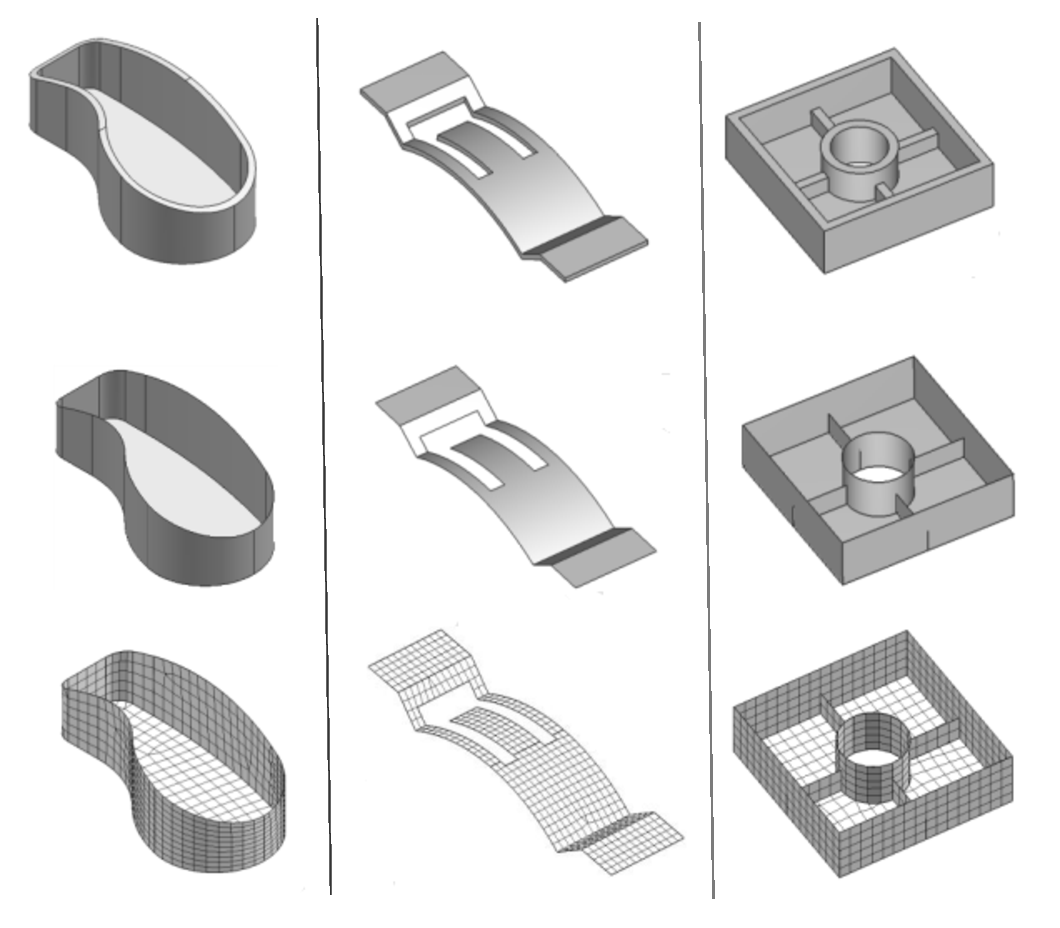
\includegraphics[width=0.75\linewidth]{..//Common/images/WooMidsurfaces.pdf}
		\caption{Thin-walled Models, Midsurfaces, Meshes (Source: Woo~\cite{Woo2013})}
		\label{fig:introduction:woomids}
	\end{figure}
	
%%\bigskip

Figure~\ref{fig:introduction:woomids} shows 3 thin-walled CAD models in the first row. The second row shows their corresponding midsurface representations. The third row shows shell meshing applied on the midsurfaces for CAE analysis. Midsurface, in different forms, such as medial objects, mid-planes, etc., are being researched for decades. Still, there is no robust, fully automated method for its computation. The reason for this unsolved problem is that there is no single, formal definition of midsurface~\cite{Ramanathan2004}. Different applications who use midsurface have different expectations about its shape, especially at the connection points. Figure~\ref{fig:introduction:midsurfaceexptations} shows how midsurface expectation varies~\cite{Woo2013}).


%%\bigskip

\def \myfigstairspcolumnwidth{0.22}

\begin{figure}[h!]
\centering     %%% not \center
\subfloat[Model]{\label{fig:introduction:stairsmodel}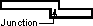
\includegraphics[width=\myfigstairspcolumnwidth\linewidth]{../Common/images/Stairs_part_2.pdf}} \quad
\subfloat[Gradual]{\label{fig:introduction:stairsfl}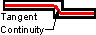
\includegraphics[width=\myfigstairspcolumnwidth\linewidth]{../Common/images/Stairs_follows_2.pdf}}  \quad
\subfloat[Mimicking]{\label{fig:introduction:stairsmk}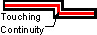
\includegraphics[width=\myfigstairspcolumnwidth\linewidth]{../Common/images/Stairs_mimic_2.pdf}}   \quad
\subfloat[Disjoint]{\label{fig:introduction:stairsseparate}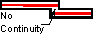
\includegraphics[width=\myfigstairspcolumnwidth\linewidth]{../Common/images/Stairs_separate_2.pdf}}
\caption{Midsurface Configurations for a Given Shape}
\label{fig:introduction:midsurfaceexptations}
\end{figure}

%%\bigskip

Figure~\ref{fig:introduction:stairsmodel} shows a step shaped thin-walled solid CAD model represented schematically as a 2D shape. Figure ~\ref{fig:introduction:stairsfl} shows two midsurface patches being joined in a gradual manner, known as  $G_1$  i.e. tangent geometric continuity. Such midsurface is preferred for CAE analysis. Figure ~\ref{fig:introduction:stairsmk} shows a planar patch being added to join the two midsurface patches. This midsurface mimics the original model exactly and is best suited for  shape matching or retrieval kind of applications where exact representation is preferred. Figure ~\ref{fig:introduction:stairsseparate} shows midsurface patches unconnected and such output can be used where a disconnect needs to be highlighted. A closer observation will reveal that all the variations shown in Figure~\ref{fig:introduction:midsurfaceexptations} are due to the continuities between midsurface patches at the connections. These continuities are of 3 types: touching ($G_0$), tangent ($G_1$) and curvature ($G_2$ ). Continuities shown in the in Figure~\ref{fig:introduction:midsurfaceexptations} are of  types $G_1,G_0,0$ respectively. 

Although there is no single, formal definition of the midsurface, some researchers have specified it semi-formally, as below:

\begin{mydef}\label{def:midsram}
Mid-surface is an aggregation of surface patches (where each patch corresponds to a pair of nonadjacent surface patches (faces) in the object that are closest to each other) that form a closed and connected set and that satisfy homotopy (Ramanathan~\cite{Ramanathan2004}).
\end{mydef}

\begin{mydef}\label{def:midsrez}
Midsurface is expressed as contiguous flow of the input solid's shape (Rezayat ~\cite{Rezayat1996}).
\end{mydef}

Primary usage of midsurface is in the CAE analysis of thin-walled parts models for placing surface elements such as ``shell'' elements.
%The present research work proposes mimicking, i.e. $G_0$ continuity output (Figure~\ref{fig:introduction:stairsmk}) as it represents the input shape faithfully. The proposed method can cater to other variations as well by incorporating with additional connection rules. These enhancements are for the future scope.  So, the primary objective of the present research work is to devise an approach to computed a well-connected midsurface mimicking the input model faithfully, in both, geometry and topology.
%%In CAE, detailed CAD model is not used as is (Section~\ref{sec:intro:cadcae}), but it is preprocessed by `Model Simplification'~\cite{DengBrittonLamTorMa2002,Lee2005,Lee2009,Lam} (Figure~\ref{fig:introduction:ModelSimplification}).
%%
%%%%\bigskip
%%
%%	\begin{figure} [!h]
%%		\centering
%%		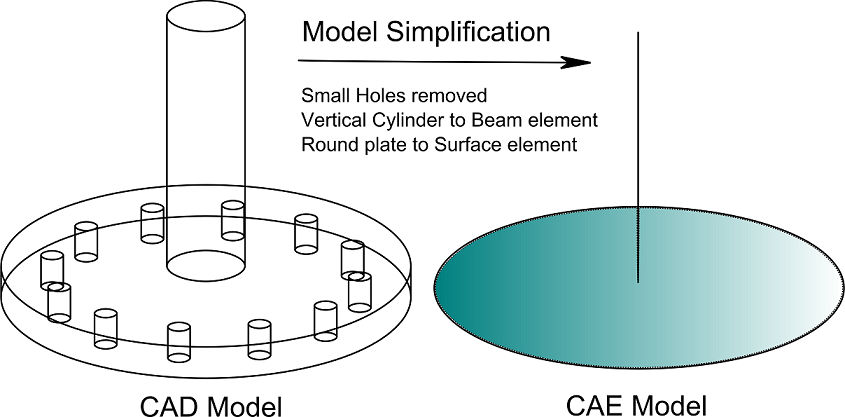
\includegraphics[width=0.6\linewidth]{..//Common/images/ModelSimplification.png}
%%		\caption{Model Simplification}
%%		\label{fig:introduction:ModelSimplification}
%%	\end{figure}
%%
%%%%\bigskip
%%
%%	Model Simplification, according to Hamri~\cite{Hamri2005}, is classified into:
%%	\begin{itemize}[noitemsep,topsep=2pt,parsep=2pt,partopsep=2pt]
%%	\item  \textbf{Skin Details}: Removal does not change 3D manifold property, like fillets, chamfer, etc.
%%	\item  \textbf{Topological Details}: Removal changes solid model topology, like, through holes etc.
%%	\item  \textbf{Dimensional Details}: Idealization, such as lines for long slender bar, midsurface for plates.
%%	\item  \textbf{Simplification Features}: User defined features to be removed.
%%	\end{itemize}
%%
%%Similarly, Model Simplification, according to Dabke~\cite{Dabke1994}, can be classified into two sub-processes, namely, Global and Element Idealization. The global idealization deals with suppressing irrelevant features and takes advantage of the symmetry to analyze only a portion of the model (also known as ``Defeaturing'' \footnote{``Defeaturing'' and ``Simplification'' have  been used interchangeably in this work, unless specified otherwise. ``Model Simplification'' is far more encompassing term, having both defeaturing and dimension-reduction, along with a few other techniques.}).  In the element idealization, shapes like slender-bar, thin-wall are converted into lower dimension geometries like midsurface. 
These elements are considered superior over solid elements, such as hex (Hexahedral) or tet (Tetrahedral), as they are computationally faster and still deliver fairly accurate analysis results. 
%In many applications, reducing the dimensions of CAD models is beneficial. For example, consider a thin plate of uniform thickness. If we model this plate using shell elements (2D surface), there will be a negligible effect on the accuracy of the CAE analysis but the computational time will reduce dramatically. Hence, dimensional reduction is studied by the physics-based simulation community (especially finite element analysts) for model simplification purposes~\cite{Thakur2009}.
%Shell elements best represent parts whose walls are `much' thinner than their typical feature size~\cite{Subrahmanyam2012}. 
%Although criterion for ``thinness'' depends on the application domain, $L/t > 20$ can be a generic consideration~\cite{Cosmos2006}.  
%%\bigskip

\begin{figure} [!h]
\centering
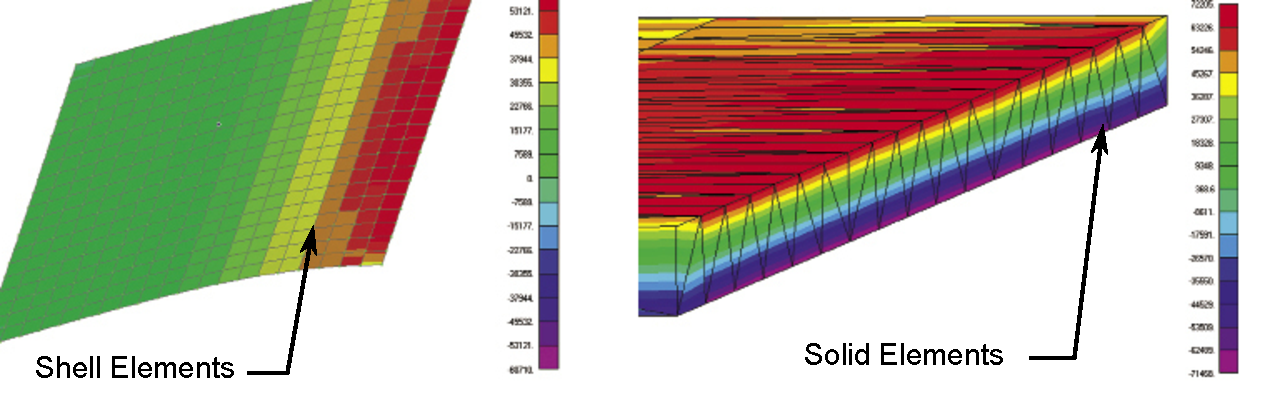
\includegraphics[width=0.95\linewidth]{..//Common/images/solidshelldesk.pdf}
\caption{Comparison of CAE Analysis with Solid and Shell Elements (Source: Cosmos~\cite{Cosmos2006})}
\label{fig:introduction:solidshell}
\end{figure}
	
%%\bigskip

Figure~\ref{fig:introduction:solidshell}  shows CAE analysis results plots of a simple plate structure. The first figure shows the result with shell elements and the second shows with tet elements. Shell elements give peak bending stress and tip deflection, very close to the theoretical calculations. Tet elements give good deflection values, but poor stress values. The tet mesh is only one element deep. To get accurate stress values, the tet element mesh needs to be at least three elements deep. To avoid the high aspect ratios, in a sample case this may drive the tet element count up towards 1 million, vs. 400 for the shell elements mesh~\cite{Abbey2013}. Thus shell element mesh is far superior in analyzing thin-walled models. A well-connected midsurface is a critical requirement for placing the shell elements.

In some cases, even for relatively thick portions, analysts use midsurface as it gives them the flexibility to play with the thickness which is not possible in case of 3D elements. While solid elements could be used for thin-walled parts, and often are, they are inefficient since many more solid elements are required to capture the same response a shell mesh can. At worst, if too few solid elements are used in a bending dominant condition, the results may appear to be correct but could be overly stiff. So, for thin-walled parts shell elements on midsurface are preferred\cite{Cosmos2006}.
	
Although there are many approaches to generate the midsurface, following section details a representative, traditional and one of the most popular approach of generating midsurface.
	
\section{Traditional Approach for Generating Midsurface}

\todo{Review comment: Get into these section with 1/2 lines as intro. Then enumerate typical steps for traditional approach and then start commentary on reported research on those steps. [DONE]}

Midsurface generation is one of the sub-types of dimension reduction process. It, along with defeaturing, forms overall ``Model Simplification'' process, which is performed during preprocessing of CAD model for CAE analysis. Traditionally, both, defeaturing and dimension reduction, are done together, one after another.

%%Approaches to generate midsurface have been part of research and commercial applications for decades. As seen in Section~\ref{sec:intro:cadcae}, these dimension reduction approaches are part of a larger process called ``Model Simplification''. Approaches for Model Simplification vary substantially, depending on the input type, such as faceted mesh model, Brep CAD model, feature-based CAD model, etc.\cite{Lam1992, Thakur2009, Yogesh2010}. 

\todo{Review comment: Can you not combine model simplification \& defeaturing?. [MODEL SIMPLIFICATION ACTUALLY COMBINES DEFEATURING AND DIMENSION REDUCTION IE MIDSURFACE. THIS PARAGRAPH IS ABOUT REMOVING IRRELEVANT FEATURES SO NAMED AS DEFEATURING]}

Figure~\ref{fig:introduction:hamdimids} shows a representative approach, a schematic outline of overall model simplification process presented by Hamdi~\cite{Hamdi2005, Hamdi2007, Hamdi2009, Hamdi2010, Hamdi2012}.
%% with following phases:
%%
%%\begin{enumerate}[noitemsep,topsep=2pt,parsep=2pt,partopsep=2pt]
%%\item  Identification of features in the input Brep or mesh model.
%%\item Identification of features to be removed, based on heuristic rules.
%%\item Generation of midsurface patches and then joining them together.
%%\item Validation of the output midsurface.
%%\end{enumerate}

%%\bigskip

	\begin{figure} [!h]
		\centering
		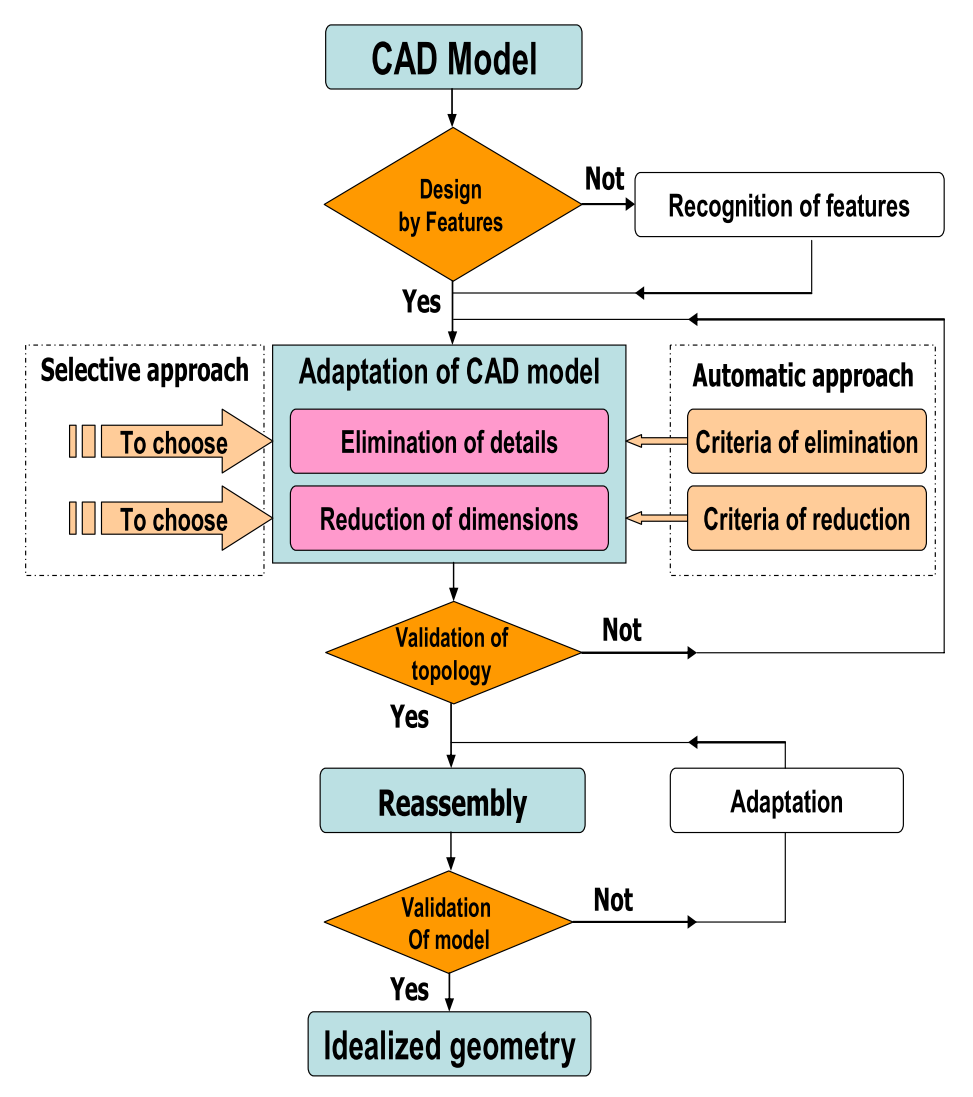
\includegraphics[width=0.75\linewidth]{..//Common/images/BlockDiagramSampleHamdi}
		\caption{Model Simplification Approach (Source: Hamdi~\cite{Hamdi2005})}
		\label{fig:introduction:hamdimids}
	\end{figure} 

%%\bigskip

CAD model is the input to this approach. It can be either feature based (denoted as ``Design by Features'' in~\ref{fig:introduction:hamdimids}) or non-feature based (i.e. Brep model). If it is Brep model, then it undergoes feature recognition process to identify features, thereby making it `feature-based CAD model'.  At the ``Model Simplification'' stage (called ``Adaption of CAD model'' in Figure~\ref{fig:introduction:hamdimids})), both defeaturing (called ``Elimination of details'') and midsurface generation (called ``Reduction of dimensions'') are performed together, one after another. In defeaturing, irrelevant features are removed, with `irrelevance' specified by `Criteria of elimination'. In dimension-reduction midsurface is generated, with `thin-walled' portions selected based on `Criteria of reduction'. The output midsurface is validated and if successful, (shown as as `Idealized geometry') sent to further downstream applications.

Figure~\ref{fig:introduction:tradmidsurfgen} shows another traditional approach with more details of actual midsurface generation process. The input CAD model (called ``Solid Model'') is defeatured in the second stage (called ``Simplification''). Here, irrelevant features such as small fillets, chamfers, etc. are removed. Midsurface computation is done using Face pairing approach. The  third stage (called ``Pair Detection'') shows how opposite faces are detected and their face pairs are formed. In the fourth stage, midsurface patches are generated. Patches are then trimmed or extended to meet at common edge. The midsurface patches are then stitched to form the final, well-connected, midsurface model.

%%\bigskip

	\begin{figure} [!h]
		\centering
		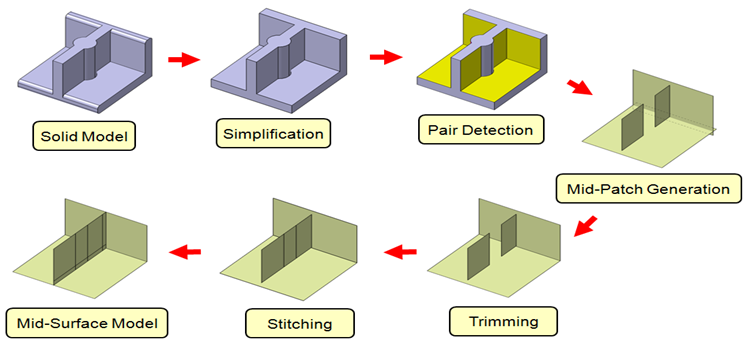
\includegraphics[width=0.9\linewidth]{..//Common/images/MidsurfaceProposedApproach}
		\caption{Traditional Midsurface Generation Approach (Source: Sheen~\cite{Sheen2005})}
		\label{fig:introduction:tradmidsurfgen}
	\end{figure} 

%%\bigskip

Both traditional approaches show the sequential execution of defeaturing and midsurface generation, as part of model simplification process. Finally, the output midsurface is validated for correctness. The following sections detail the state of the art for all of these.

\section{CAD Model Defeaturing Approaches} \label{sec:survey:defeat}

Humans, while looking at an object, at the first glance perceive its overall, gross shape and then eventually look into more details as needed~\cite{LeeLee1998}. Gross shape is the principal shape that ``represents'' the given shape, but with far lesser features. In the context of CAD-CAE the gross shape is achieved by defeaturing. Defeaturing is the process of simplification of the shape, by removing small and irrelevant feature details,  based on certain predefined objectives or criteria. It is primarily used in CAE analysis where such simplified models lower the complexity of the finite element mesh and thus reduce the analysis time. It is also used in shape matching \& retrieval, fast visualization, hiding proprietary details, transmission across the network, etc. 

\todo{Review comments: What are refs? [REMOVED BOTH DEFINITIONS]} 

% \replaced{The present research}{This} work focuses on using defeaturing for finding the gross shape needed in the computation of well-connected midsurface. 	
	
%%Grossness depends on the size criteria or threshold. Details having sizes below the threshold are removed. With lesser irrelevant details on the input model, the generated midsurface becomes far more representative of the input model and is robust (any small change in the input model shape does not affect the output midsurface in any appreciable manner).
	
Traditionally, defeaturing has largely been a manual and tedious task. Small and irrelevant features are first recognized in the input mesh or Brep CAD model and are removed manually~\cite{BelazizBourasBrun2000}. Users view this task as too extensive and resort to recreate the necessary geometry than to simplify the existing one~\cite{Halpern1997, Abbey2013,Lam,Lee2005, Lee2009}.  
	
%In the \replaced{traditional }{current CAD-CAE applications, many} simplification methods recognize small, irrelevant features on a mesh or a solid body first, then remove them to get the simplified (called ``defeatured'')  model~\cite{}. 

\deleted{Instead, if a feature based CAD model is used as an input, then it has the advantage of the availability of ready features, so that the suppression and healing becomes relatively straightforward and robust. In such a feature based defeaturing method, the primary challenge is the identification of the suppressible features.
 In the past, the suppressibility used to be based on some insufficient criteria, like using full feature parameters, selecting all the negative features, etc. The objective of this work is to use far more accurate criteria and develop a computational method to automatically find the simplified geometry of a sheet metal part model which can be used for further computations such as the generation of the midsurface (more details in the Chapter~\ref{ch:Defeaturing}).} Feature-based defeaturing approaches can be classified as:

\begin{enumerate}[noitemsep,topsep=2pt,parsep=2pt,partopsep=2pt]
	\item CAD Model Defeaturing based on Feature Information.
	\item CAD Model Defeaturing based on Feature Recognition.
	\item CAD Model Defeaturing based on Decomposition.
\end{enumerate}

Following section elaborates theses approaches in details. \deleted{This research uses defeaturing of the feature based CAD model, using decomposition as well as feature data, thus their state-of-the-arts are presented below.} 

\todo{Review comments: Delete. [WITH THIS DELETION THE CONTINUITY IS GONE. RESTORE BACK?]}

\subsection{CAD Model Defeaturing Based on Feature Information}

Thakur et al.~\cite{Thakur2009} surveyed and classified various model simplification approaches into four categories, such as surface-based, volume-based, feature based, and dimension-reduction. First three categories are about defeaturing and the fourth is for midsurface generation. \added{From this survey it is observed that} most methods were based on the mesh and Brep model as the input, with very few based on the feature based CAD model. 

In feature-based CAD, model is built step by step using feature modeling operations. The history of modeling operations is represented in the form of feature tree.

%%\bigskip

	\begin{figure} [!h]
		\centering
		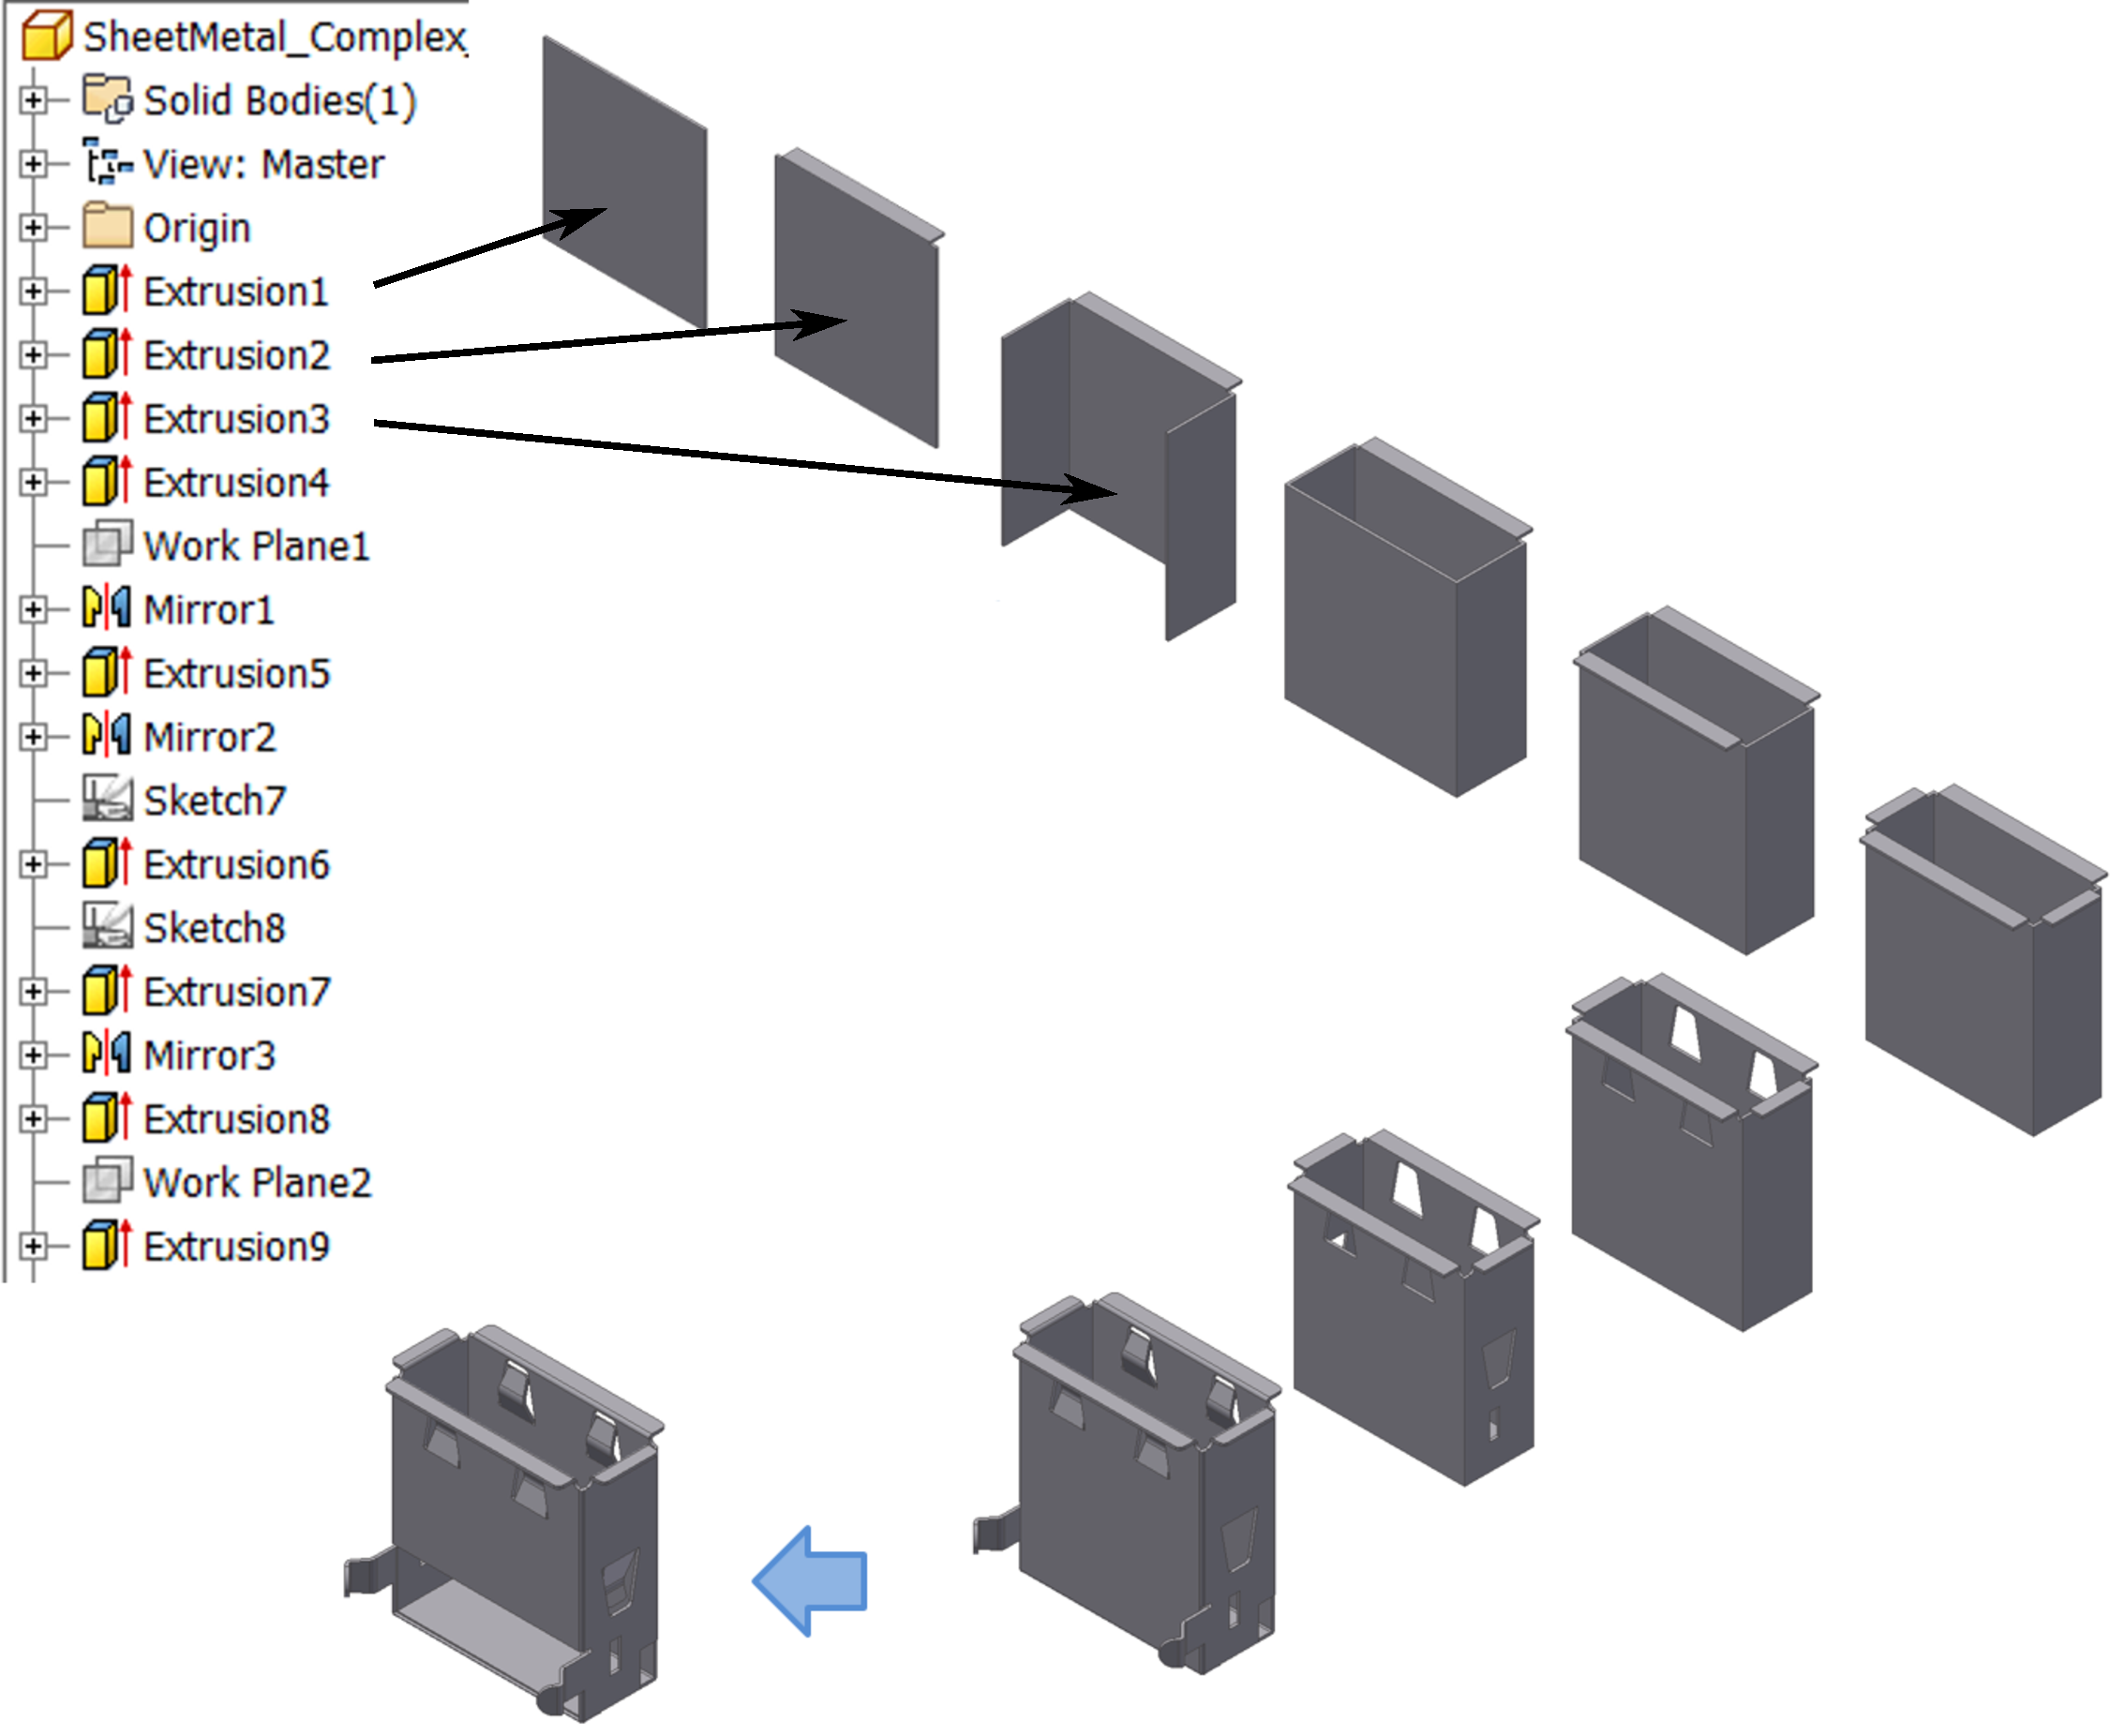
\includegraphics[width=0.75\linewidth]{..//Common/images/usbfeaturetree_arrow.pdf}
		\caption{Construction of USB CAD Model by Features}
		\label{fig:introduction:usbtree}
	\end{figure} 

%%\bigskip

Figure~\ref{fig:introduction:usbtree} shows construction of a CAD model of a USB part using a variety of modeling features. At each stage, a new feature gets added to or subtracted from the model built till then. The feature tree is shown at the left. Feature based CAD model, internally builds the model in Brep format as well. So, the final shape, shown at the bottom can be exported in the Brep format. Non-feature based CAD models create Brep format directly and are not built using features. So, features are not accessible from Brep formats.

One of the critical advantage of feature-based CAD model over Brep CAD models is that the individual features can be removed and the model can be regenerated to a valid model \replaced{without }{sans} those removed feature. Thus, feature based CAD models present clear advantage over Brep, for defeaturing. \added{Kang~\cite{Kang2013} observed and reported that} feature-based CAD defeaturing operations have better applicability than mesh or Brep model based simplification methods for product design and engineering applications.\deleted{Ready APIs (Application Programming Interfaces) are available to exclude certain features while computing the final shape.} 

Some of the notable feature based CAD defeaturing approaches are reviewed below:
 
Dabke~\cite{Dabke1994} through the concept of  `global idealization', was one of the first researchers to leverage feature information for defeaturing. His method was based on expert system with heuristic rules derived from the analyst's experience. His approach was \added{however} rudimentary in the usage of features.

%%Joshi and Dutta~\cite{Joshi2003}  recognized the sheet metal features on free-form surfaces and then suppressed them for simplification. Their work was limited to only holes, fillets and bosses.
%%
%%Lee~\cite{Lee2005, SangHunLee2005, Lee2009} elaborated a method to reorder features in the history tree and then to re-execute the history of the reordered features up to the given level of details (LoD). Since the model re-evaluation is computationally intensive, he used the cellular topology (CT) for increasing the performance. One of the major limitations of this approach is that once the model is converted to CT, its feature update capability would cease to exist, making it difficult for any further modifications.
	 
 Smit~\cite{Smit2009} surveyed various approaches for CAD-CAE integrations and concluded that since features carry domain-specific information, they can bring context-relevant defeaturing. But, the limitation is, many features are built using entities from the existing features, creating dependencies called "parent-child" relationships. Removing the parent feature removes the child features too. Thus, deciding the eligibility of removal of the feature should include similar evaluation of child features also. Otherwise, one has to build or adopt the part in such a way that the dependencies are removed or rerouted~\cite{AmesRiveraWebbHensinger1997}.

%%Woo~\cite{Woo2009} proposed a method to recognize subtractive features on Brep model, thus eliminating the problem of looking at the history tree. This approach lacked coverage in terms of variety of features being recognized and thus, was limited to simple shapes

Hamdi et al.~\cite{Hamdi2012a} surveyed defeaturing techniques and classified them based on the input format, features simplified, defeaturing criterion, advantages, limitations and application domain. Most of the methods were Brep-based and removed features like holes, chamfers, fillets, protrusions, depressions, passages, concave regions, etc. They used size threshold as well as application-specific rules for identification of the removable features.  

Russ~\cite{Russ2012} mentioned that the determination of the non-critical (suppressible) features relies on different attributes of not only the features themselves, but also of the entire part model and analysis. Some of these attributes include the feature type, feature dimensions, proximity of features to the boundary conditions, analysis type, and part dimensions. He used full feature parameters for deciding the eligibility of the removal. 

\deleted{The selection criteria for suppressing the features, apart from being application-specific, are based on the targeted accuracy, cost or preparation time, etc~\cite{Danglade2013}. Looking at the variety of inputs, types of analysis and application domains, it is difficult to quantify and generalize. So, each domain typically presents its own feature taxonomy with regards to defeaturing to decide the eligibility for suppression.}
	
	Danglade~\cite{Danglade2013} used machine-learning techniques to capitalize the knowledge and experience of CAE analysts for defeaturing. After a large number of learning trials, the system itself became capable of deciding relevance of features. This approach requires feeding of huge initial data to be effective for usage as real life applications.

	Kang et al.~\cite{Kang2013} customized the defeaturing criteria for shipyard requirements where, apart from geometric reasoning criteria such as volume, they included application-specific rules related to ports and outer boundary of the model.
	
Thus, for feature based CAD model defeaturing, although having ready access to features reduces the complexity of removal and regeneration of the model, the `selection of feature for removal' itself remains a challenge. In case of mesh or Brep CAD models, as seen in Figure~\ref{fig:introduction:hamdimids}, they do not have ready access to features, thus need to undergo feature recognition process to populate the features. Then, these features are evaluated for removal. Following section reviews defeaturing approaches based on Feature Recognition.
	
\todo{Review comment: I think we have a separate section. [DONE.``Commercial Applications'' SECTION]}

\deleted{Commercial packages like ACIS\textsuperscript{\textregistered}, Autodesk Fusion\textsuperscript{\textregistered}, Altair's Hypermesh\textsuperscript{\textregistered} also to provide similar defeaturing capabilities mainly for CAE analysis.} 

\todo{Review comment: Can you combine all defeaturing related research into one table. [DONE]}

%%Below is the summary of the relevant FCAD defeaturing approaches: 
 
%%\csvreader[longtable=|p{0.15\linewidth}|p{0.1\linewidth}|p{0.2\linewidth}|p{0.2\linewidth}|p{0.17\linewidth}|p{0.17\linewidth}|,
%%    table head=\toprule \bfseries Author & \bfseries Input& \bfseries  Method & \bfseries  Approach& \bfseries  Advantages& \bfseries  Limitations \\ \midrule \endhead,% \bottomrule \endfoot,
%%  late after last line=\\\bottomrule,
%%  before reading={\catcode`\#=12},after reading={\catcode`\#=6},    
%%    late after line=\\\hline]%
%%{../DocsSources/litsurvey_fbd_defeature.csv}{Author=\Author, Input=\Input, Method=\Method, Approach=\Approach, Advantages=\Advantages ,Limitations=\Limitations}%
%%{\Author  & \Input&  \Method &\Approach & \Advantages & \Limitations}%
	
\todo{Review comment: But where are the defeaturing techniques? Next two sections not needed. [REMOVED LIT SURVEY OF SHEET METAL FEATURE TAXONOMY AS IT WAS NOT ABOUT EXISTING DEFEATURING TECHNIQUES]}	

%%\subsubsection{Sheet Metal Feature Taxonomy}
%%
%%	The research presented here focuses on feature based defeaturing specific to sheet metal parts. Sheet metal parts are prevalent in industries, such as automotive, aerospace, process, electronics, etc.  Clear definition and classification of sheet metal features is a prerequisite in deciding the defeaturing rules. Some of the available classifications for sheet metal feature based CAD models (SMFCAD) are reviewed in the following section. 
%%	
%% Liu et al.~\cite{Liu2004} stated that a sheet metal CAD part model is made up of base features (Wall/Face feature) upon which several child/secondary features (Cutouts, etc.) are positioned. Then, the tertiary and connector features are added to complete the desired shape. They classified sheet metal features into Primitives features which are independent features, Add-ons which are on the Primitives, Connectors which connect the features and Composites which are made up of the earlier-defined types.
%%
%%Sunil~\cite{Sunil2008} classified sheet metal features into face-based features which lie on the face (holes, dimple, and beads), edge-based features (flange, ridge) which lie on the periphery of the part, while transitive features (bend) lie between the faces.
%%
%%Below is the summary of the relevant Sheet Metal Features classification approaches:
%% 	
%%\csvreader[longtable=|p{0.15\linewidth}|p{0.13\linewidth}|p{0.2\linewidth}|p{0.2\linewidth}|p{0.17\linewidth}|p{0.17\linewidth}|,
%%    table head=\toprule \bfseries Author & \bfseries Input& \bfseries  Method & \bfseries  Approach& \bfseries  Advantages& \bfseries  Limitations \\ \midrule \endhead,% \bottomrule \endfoot,
%%  late after last line=\\\bottomrule,
%%  before reading={\catcode`\#=12},after reading={\catcode`\#=6},    
%%    late after line=\\\hline]%
%%{../DocsSources/litsurvey_sheetmetal_taxonomy.csv}{Author=\Author, Input=\Input, Method=\Method, Approach=\Approach, Advantages=\Advantages ,Limitations=\Limitations}%
%%{\Author  & \Input&  \Method &\Approach & \Advantages & \Limitations}% 	
%%
%%Survey suggests that for a well-connected midsurface, primitive and connecting/transitive features are critical and they need to be retained, whereas secondary features can be suppressed by comparing their size relative to the given threshold. 
%%
%%
%%\subsubsection{Sheet Metal Feature-recognition}
%%
%%Mesh and Brep are two of the most commonly used data model to represent CAD solids. Feature recognition (FR) approaches are used to identify Sheet Metal features.
%%
%%Sunil~\cite{Sunil2008} tackled the problem of features interaction  through  a  hybrid  approach  for  feature recognition that is both graph and rule based.  He classified features as Face-based (holes, dimple, and beads), edge-based features (flange, ridge) and transitive features (bend).
%%
%%Ravi Kumar Gupta~\cite{Gupta2008}~\cite{Gupta2013} ~\cite{Gupta2013a} recognized deformation features as a set of faces classified by type and nature and then applying rules.
%%
%%Kannan and Shunmugam ~\cite{Kannan2009} classified into four major classes cut, stretched, drawn and bent, by developing rules on the midsurface of the sheet metal part. Drawback of this approach is that the quality FR depends highly on the quality of input midsurface.
%%
%%Below is the summary of the relevant Sheet Metal Features recognition approaches:
%%
%%
%%\csvreader[longtable=|p{0.15\linewidth}|p{0.14\linewidth}|p{0.2\linewidth}|p{0.2\linewidth}|p{0.17\linewidth}|p{0.17\linewidth}|,
%%    table head=\toprule \bfseries Author & \bfseries Input& \bfseries  Method & \bfseries  Approach& \bfseries  Advantages& \bfseries  Limitations \\ \midrule \endhead,% \bottomrule \endfoot,
%%  late after last line=\\\bottomrule,
%%  before reading={\catcode`\#=12},after reading={\catcode`\#=6},    
%%    late after line=\\\hline]%
%%{../DocsSources/litsurvey_fr_sheetmetal.csv}{Author=\Author, Input=\Input, Method=\Method, Approach=\Approach, Advantages=\Advantages ,Limitations=\Limitations}%
%%{\Author  & \Input&  \Method &\Approach & \Advantages & \Limitations}%
%%
%% 	
%%	
%%\subsubsection{Feature-recognition-based Defeaturing}

\subsection{CAD Model Defeaturing Based on Feature Recognition}

Mesh and Brep are widely used data formats to represent CAD models. In the context of defeaturing, they lack much needed ready access to features. Feature recognition (FR) approaches are used to identify small-irrelevant features in them, which are then evaluated for removal. 

Even in case of feature based CAD modeling paradigm, single shape can be modeled with two different feature sequences. So, the feature trees may be different for similar shape. Defeaturing based on features, along with different dependencies, may yield different results. To achieve consistent defeaturing results independent of the modeling history, some attempts use just the final Brep model, and then recognize the features~\cite{Woo2009} to be removed directly from that final model.	

Sandia report~\cite{Watterberg1999} recognized features like holes, fillets and chamfers on mesh model and suppressed the smaller ones. In one of the test-cases, the report observed that, the polygon mesh count reduced 10 times. One of the drawback of the approach presented was that it did not incorporate application or domain specific rules for removal of the features.

Belaziz et al.~\cite{BelazizBourasBrun2000} proposed morphological analysis of Brep models based on recognition of form features and using their transformations for simplifications and idealizations. They constructed gross shape step by step by detecting form features. 

Joshi Datta ~\cite{Joshi2003} recognized features such as holes-fillets-bosses based on type of free form surfaces. Their approach was limited in the features it could recognize.

Hamdi et al. ~\cite{Hamdi2005}~\cite{Hamdi2007} ~\cite{Hamdi2009} ~\cite{Hamdi2010}~\cite{Hamdi2012}~\cite{Hamdi2012a} eliminated details by merging faces. They also took into account CAE input such as load path BCs. Their method was simplistic in both defeaturing and idealization.

Woo~\cite{Woo2009} proposed a method to recognize subtractive features on Brep model, thus eliminating the problem of looking at the history tree. This approach lacked coverage in terms of variety of features being recognized and thus, was limited to simple shapes

Recognizing features on mesh or Brep CAD model is challenging and often resorts to heuristic rules, making it error prone. It does not work well in real-life parts having various features are interacting with each others. Following subsection evaluates defeaturing by decomposing the input model into primitive shapes and then performing defeaturing.

%%Below is the summary of the relevant Feature-recognition-based Defeaturing approaches:
%%
%%\csvreader[longtable=|p{0.15\linewidth}|p{0.14\linewidth}|p{0.2\linewidth}|p{0.2\linewidth}|p{0.18\linewidth}|p{0.17\linewidth}|,
%%    table head=\toprule \bfseries Author & \bfseries Input& \bfseries  Method & \bfseries  Approach& \bfseries  Advantages& \bfseries  Limitations \\ \midrule \endhead,% \bottomrule \endfoot,
%%  late after last line=\\\bottomrule,
%%  before reading={\catcode`\#=12},after reading={\catcode`\#=6},    
%%    late after line=\\\hline]%
%%{../DocsSources/litsurvey_fr_defeature.csv}{Author=\Author, Input=\Input, Method=\Method, Approach=\Approach, Advantages=\Advantages ,Limitations=\Limitations}%
%%{\Author  & \Input&  \Method &\Approach & \Advantages & \Limitations}%
	

\subsection{CAD Model Defeaturing Based on Decomposition}

Decomposition is one of the most effective methods for reducing the complexity of the model~\cite{Zhu2015}. Brep, being one the most commonly used modeling format to represent solids in CAD, volume-based methods are used on Brep solid model to decompose it into sub-solids. In volume based decomposition methods, the input solid is partitioned by cutting planes. Cutting planes are selected based on the application requirement. Certain applications need Convex Partitioning, where cutting planes are placed at concave edges, such that, after partitioning, the sub-solids obtained are of convex type. 

%%\bigskip

	\begin{figure} [!h]
		\centering
		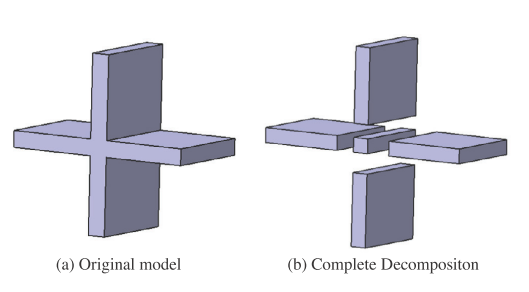
\includegraphics[width=0.6\linewidth]{..//Common/images/zhudecomp}
		\caption{Convex Partitioning (Source: Zhu~\cite{Zhu2016})}
		\label{fig:introduction:zhudecomp}
	\end{figure} 

%%\bigskip

Figure~\ref{fig:introduction:zhudecomp} shows convex partitioning of the input solid shape, mentioned as ``Original model'' into convex sub-solids, shown under ``Complete Decomposition''. 
Decomposition has been used effectively for featuring. Some of the salient approaches are mentioned below.

Sang Hun Lee~\cite{Lee2005, SangHunLee2005, Lee2009} elaborated a method to reorder features in the history tree and then to re-execute the history of the reordered features up to the given level of details (LoD). Since the model re-evaluation is computationally intensive, he used the cellular topology (CT) for increasing the performance. One of the major limitations of this approach is that once the model is converted to CT, its feature update capability would cease to exist, making it difficult for any further modifications.

Yoonhwan Woo~\cite{Woo2009} proposed a method to recognize subtractive features on Brep model, thus eliminating the problem of looking at the history tree. This approach lacked coverage in terms of variety of features being recognized and thus, was limited to simple shapes.

Byung Chul Kim~\cite{Kim2014} generated  feature based model by Cellular or Wrap or Split or Feature decomposition and then suppressed by type and size. This method can be applied widely but was limited in the recognition capabilities.

Decomposition, like feature-recognition, is highly heuristic and error prone, especially for complex models. Thus, defeaturing using decomposition, has limitations while using for real life complex part models.

%%Below is the summary of the relevant decomposition-based Defeaturing approaches:
%%
%%\csvreader[longtable=|p{0.15\linewidth}|p{0.1\linewidth}|p{0.2\linewidth}|p{0.2\linewidth}|p{0.17\linewidth}|p{0.17\linewidth}|,
%%    table head=\toprule \bfseries Author & \bfseries Input& \bfseries  Method & \bfseries  Approach& \bfseries  Advantages& \bfseries  Limitations \\ \midrule \endhead,% \bottomrule \endfoot,
%%  late after last line=\\\bottomrule,
%%  before reading={\catcode`\#=12},after reading={\catcode`\#=6},    
%%    late after line=\\\hline]%
%%{../DocsSources/litsurvey_decomp_defeature.csv}{Author=\Author, Input=\Input, Method=\Method, Approach=\Approach, Advantages=\Advantages ,Limitations=\Limitations}%
%%{\Author  & \Input&  \Method &\Approach & \Advantages & \Limitations}%

Table~\ref{tbl:survey:alldefeature} presents the summary of all the above mentioned CAD Model Defeaturing Approaches:

\todo{Review comment: Merge all tables together. [DONE]}

%%\bigskip

\csvreader[longtable=|p{0.15\linewidth}|p{0.1\linewidth}|p{0.15\linewidth}|p{0.15\linewidth}|p{0.17\linewidth}|p{0.17\linewidth}|,
    table head=\toprule \bfseries Author & \bfseries Input& \bfseries  Method & \bfseries  Approach& \bfseries  Advantages& \bfseries  Limitations \\ \midrule \endhead \caption{CAD Model Defeaturing Approaches}\label{tbl:survey:alldefeature} \endlastfoot,% \bottomrule \endfoot,
  late after last line=\\\bottomrule,
  before reading={\catcode`\#=12},after reading={\catcode`\#=6},    
    late after line=\\\hline]%
{../DocsSources/litsurvey_all_defeature.csv}{Author=\Author, Input=\Input, Method=\Method, Approach=\Approach, Advantages=\Advantages ,Limitations=\Limitations}%
{\Author  & \Input&  \Method &\Approach & \Advantages & \Limitations}%


%%\bigskip

\subsection{Observations on CAD Model Defeaturing Approaches}\label{sec:litsurvey:obsdefeat}

\todo{Review comments: Do not directly put bullets. Give some precursor, enumerate or just write verbose summary. [ADDED FEW LINES. REMOVED CITATIONS]}

\added{Research in defeaturing approaches has been going on for decades and remains a challenging problem to solve. Varied requirements from different domains, complexities of the parts and critical role of engineering judgment in the selection rules, has made defeaturing a challenge. Following is the list of some of the important observations from the survey of above CAD model defeaturing approaches:}

\begin{enumerate}[noitemsep,topsep=2pt,parsep=2pt,partopsep=2pt]
	\item Most defeaturing approaches take either Brep or mesh as input CAD model. Small irrelevant features are recognized and removed. Feature recognition, being a heuristic methodology, is not successful on many complex parts. Thus, success of defeaturing is limited and non-deterministic.
	\item In case of feature based CAD models, due to ready access to features, removal of irrelevant features and subsequent regeneration of the model is easier. The challenge remains in selection of features to be removed.
	\item Size based defeaturing, where features below certain size threshold are removed, is the most prevalent approach. Apart from this, few approaches suggest use of application specific engineering judgment as well, such as, holes in the load path should not be removed, however small they are.
	\item Full feature dimensions are used by some of the approaches for deciding size based removal of features. Features volumes, typically are consumed partially in the model when they get added. Thus using full feature dimensions, giving wrong candidates for defeaturing.
	\item Feature dependencies across features, fetch child features which are not originally selected for removal. These dependencies should be minimized by appropriate modeling practices.
\item Identification of the irrelevant features, only by their feature types, cannot be used blindly across all domains. For example, a rib-like feature may not be relevant in the metal flow analysis, but may be relevant in the heat transfer analysis. 
\end{enumerate}

\added{It is thus, observed that CAD model defeaturing approaches largely do not leverage feature information and are not customized to application domain.}

Following section elaborates the second important aspect of the model simplification, i.e. the dimension reduction approaches, specifically the midsurface generation methods, along with their state of the art.

\section{Midsurface Generation Approaches}

Midsurface is part of a family of geometric entities known as ``Medial'' objects. Other members of the family are Medial Axis Transform, Skeleton, Symmetric Axis, etc.~\cite{Butlin2009}. A medial object represents the input solid shape with one or two dimensions less and lies midway of it~\cite{Armstrong}.  Medial objects such as skeleton and medial surface, are 2 and 1 dimension less than the input solid shape respectively.

%%\bigskip

	\begin{figure} [h]
		\centering
		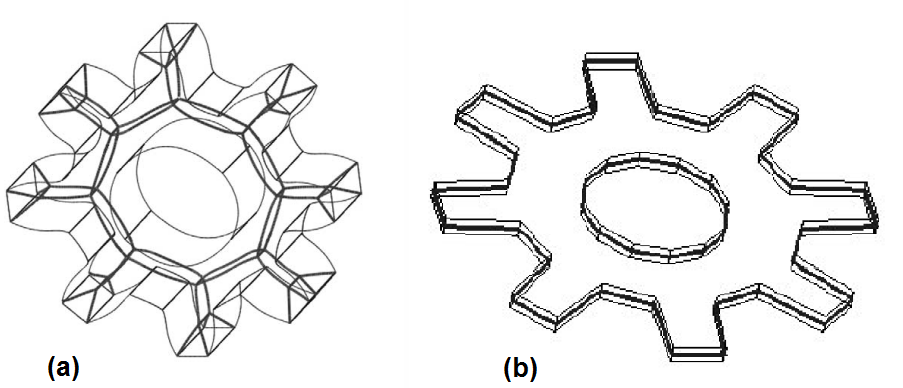
\includegraphics[width=0.7\linewidth]{..//Common/images/mat2d3d}
		\caption{Skeleton and Medial Surface of Gear Shape (Source: Ramanathan~\cite{Ramanathan2004, Ramanathan2005})}
		\label{fig:litsurvey:mat2d3d}
	\end{figure}
	
%%\bigskip	

Figure~\ref{fig:litsurvey:mat2d3d}a shows a 1D representation, called skeleton, of a 3D gear shaped solid. Figure~\ref{fig:litsurvey:mat2d3d}b shows a 2D representation, called medial surface, of a similar 3D gear shaped solid. 

Medial objects are used for different applications, such as pattern recognition, approximation, similarity estimation, collision detection, animation, matching, CAE, etc. Processing medial object is quicker as they are simpler, of lower dimensions and still represent the input shape by mimicking it faithfully. Some of the widely used medial object computation approaches are Medial Axis Transform (MAT)~\cite{Harry1967},  Chordal Axis Transform (CAT)~\cite{Prasad2007}, Thinning~\cite{Lam1992}, and Pairing~\cite{Rezayat1996}, etc.  

\todo{Review comment: In general instead of giving a terse reference of figure, it is better ti say Fig X.X indicates/depicts/shows schematic/diagrammatic representation of various media axis computation approaches. [DONE]}

%%\bigskip

	\begin{figure} [h]
		\centering
		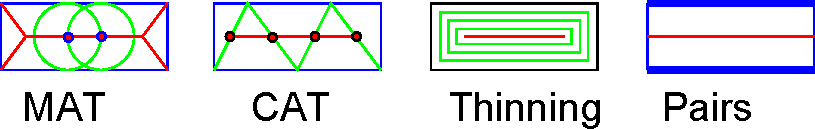
\includegraphics[width=0.7\linewidth]{..//Common/images/MedialMethodsOnlyShort.pdf}
		\caption{Medial Generation Approaches}
		\label{fig:litsurvey:medials}
	\end{figure}
	
%%\bigskip	
 
Figure~\ref{fig:litsurvey:medials} shows their schematic representations. Lines in the middle (with red color) depict medial object of an input shape represented by outer rectangle. In MAT, medial is obtained by tracing loci of the centers of maximal disk, shown as circle, traversing within the input shape. In CAT, the input shape is triangulated first, then medial is obtained by joining midpoints of the sides of the triangle. In Thinning, medial is obtained by successively offsetting the boundary of the input shape, till no further offset is possible.In Pairing, opposite geometric entities are found and their pairs are formed. Medial is computed as an entity equidistant from the paired entities.

Approaches shown in Figure~\ref{fig:litsurvey:medials} can be classified into two categories, viz. formal and heuristics. In formal approaches, a medial object is computed mathematically, in a formal manner, whereas in heuristic approaches, no such mathematical formulation is used. Medial object is computed based on empirical, rules-based procedure.
Out of the approaches shown in Figure~\ref{fig:litsurvey:medials}, MAT, CAT and Thinning are considered as formal approaches, whereas Pairing is denoted as a heuristic approach.  Following sub-sections elaborate these approaches and towards end of each category, comparison table is presented along with the summary of observations.

The formal approaches are:

\begin{enumerate}[noitemsep,topsep=2pt,parsep=2pt,partopsep=2pt]
	\item  Medial Axis Transform (MAT).
	\item Chordal  Axis Transform (CAT).
	\item Thinning and Straight Skeleton.
	\item Parametric Equations.
\end{enumerate}

The heuristic approaches are:

\begin{enumerate}[noitemsep,topsep=2pt,parsep=2pt,partopsep=2pt]
	\item Face pairing or Midsurface abstraction.
	\item Feature-based midsurface.
	\item Decomposition based midsurface.
\end{enumerate}

Following section elaborates theses approaches in details.
 
\subsection{Generating Midsurface by Medial Axis Transform (MAT)}

MAT is a locus of the center of an inscribed disc of maximal diameter as it rolls around the object interior. Figure~\ref{fig:litsurvey:mat} depicts representation of MAT in 2D (called Medial Axis Curve) as well as in 3D (called Medial Surface). Most MAT algorithms utilize Voronoi diagrams and Delaunay triangulation. 


%%\bigskip

\begin{figure}[!h]
\centering
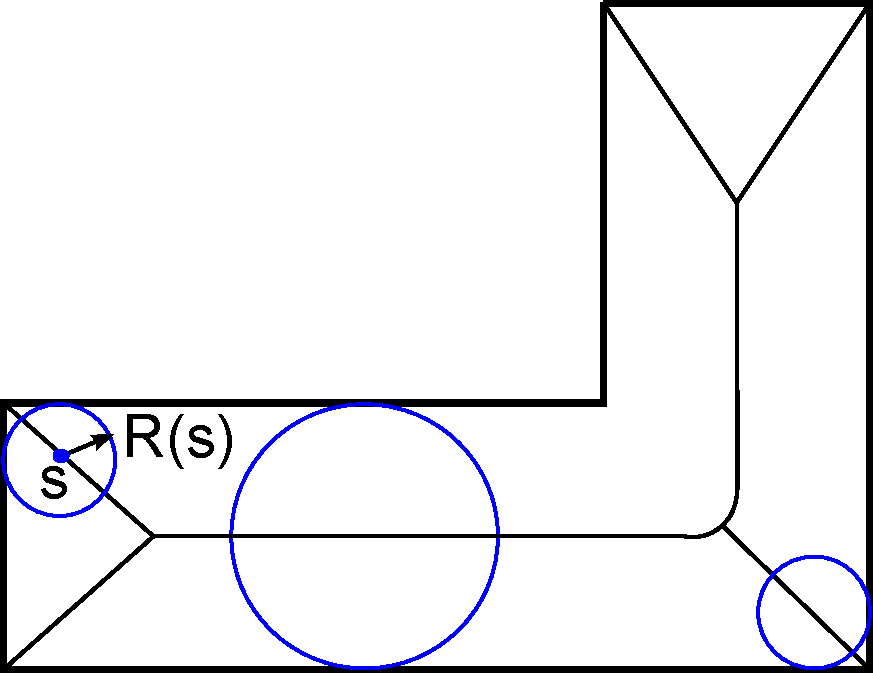
\includegraphics[width=0.3\linewidth]{../Common/images/MAT1.pdf}
\caption{Medial Axis Transform (Source: Sheen~\cite{Sheen2008})}
\label{fig:litsurvey:mat}
\end{figure}


%%\bigskip

MAT was first introduced by Blum~\cite{Harry1967} in 1967. He proposed Medial Axis Transform (MAT) as a representation that embodies the skeleton of an object as well as the width of the object at every point on the skeleton.  

Robinson~\cite{Robinson2006, Robinson2007}, Stanley~\cite{Stanley2010} used the MAT approach, either to detect thin portions or to compute midcurve. \deleted{All these approaches needed post processing to remove erroneous branches. More in-depth survey of approaches is presented by Attali~\cite{Attali2004}. }

In one of the recent approaches, Automex~\cite{Automex} used Scale Axis Transform, a modified MAT method, where rolling balls are scaled to address the issue of branches and perturbations. Although the approach is promising, it suffers limitations in complex cases where it creates unnecessary topological fragments.

Ramanathan~\cite{Ramanathan2004} pointed out that the MAT falls short in its ability to reflect the local topology of the part exactly. This is because of the extraneous portions and non-linear entities that occur due to convex and concave corners in the domain. 
%\added{Figure~\ref{fig:litsurvey:midcurve}a shows branches at corners $A,B,C,D$}. On the other hand, Figure~\ref{fig:litsurvey:midcurve}b shows mid-curve that resembles the original geometry to a greater extent. 
He modified the MAT method to remove erroneous branches. \added{Figure~\ref{fig:litsurvey:midcurve}a depicts the usual MAT output showing branches such as $A-E1,B-E1,F1-C,F1-D$, whereas Figure~\ref{fig:litsurvey:midcurve}b shows midcurve output where spurious branches have been replaced by two extension forming a continuous line, thus mimicking the original shape.}

	\begin{figure} [h]
		\centering
		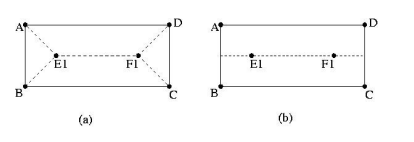
\includegraphics[width=0.7\linewidth]{..//Common/images/midcurve}
		\caption{Modified MAT for Midcurve Computation (Source: Ramanathan~\cite{Ramanathan2004} )}
		\label{fig:litsurvey:midcurve}
	\end{figure}
	
Many regularization or post-processing methods have been proposed to remove the erroneous branches \cite{Attali2004,  Tam2003, Algazi1992,Brandt1992, Ogniewicz1995, Tam2002, Turkiyyah1995,Turkiyyah1997, KaoJune1999}, but they are far from being practically useful.

\todo{Review comment: Serial refs can be stacked. [DONE]}


\todo{Review comment: Merge all th tables related to MAT, CAT Thinning etc. [DONE. COMBINED OBSERVATIONS AS WELL]}

%%Below is the summary of the relevant MAT approaches:
%%
%%\csvreader[longtable=|p{0.17\linewidth}|p{0.09\linewidth}|p{0.12\linewidth}|p{0.2\linewidth}|p{0.17\linewidth}|p{0.17\linewidth}|,
%%    table head=\toprule \bfseries Author & \bfseries Input& \bfseries  Medial& \bfseries  Approach& \bfseries  Advantages& \bfseries  Limitations \\ \midrule \endhead,% \bottomrule \endfoot,
%%  late after last line=\\\bottomrule,
%%  before reading={\catcode`\#=12},after reading={\catcode`\#=6},    
%%    late after line=\\\hline]%
%%{../DocsSources/litsurvey_mat.csv}{Author=\Author, Input=\Input, Method=\Method, Approach=\Approach, Advantages=\Advantages ,Limitations=\Limitations}%
%%{\Author  & \Input&  \Method &\Approach & \Advantages & \Limitations}%


%%\subsubsection{Observations on MAT}
%%\begin{itemize}[noitemsep,topsep=2pt,parsep=2pt,partopsep=2pt]
%%	\item Biggest strength of MAT is that it can be computed of any shape, thick or thin. Being formally defined reversal, meaning , ``given a MAT compute the original shape'', is possible.
%%	\item Major drawback of this method is that it creates unnecessary branches and its shape is smaller than the original corresponding faces.
%%	\item  MAT based approaches also suffer from robustness problem. A slight change in base geometry forces re-computation of MAT and the results could very well be different than the original.
%%	\item Although MAT approaches have been around for decades and are fairly mature, its usage in midcurve-midsurface generation is still very complex and difficult to ensure appropriate topology.
%%
%%\end{itemize}


\subsection{Generating Midsurface by Chordal  Axis Transform (CAT)}	

\todo{Review comment: What is CAT based approach. [ADDED LINES]}

For computing CAT, in case of 2D shape, the input is meshed by Constrained Delaunay Triangulation (CDT). Midpoints of the chords i.e. sides of the triangles, are joined to form the medial~\cite{QuadrosRoshanOwenBrewerShimada2004}. In case of 3D solid shape as input, a tetrahedral (tet) mesh is generated without inserting interior nodes and then midsurface is generated by fitting through midpoints of tetrahedral elements' faces, called chordal faces. Figure~\ref{fig:litsurvey:cat} shows CAT approach applied to both, 2D and 3D input shapes. Figure~\ref{fig_cat2d} shows how 2D input  shape is meshed with triangles and then a curve is fitted through the midpoints of the triangle edges (chords). Figure~\ref{fig_cat3d} shows result of tetrahedral elements meshing and computation of CAT by fitting a surface through midpoints of the tetrahedral elements faces (chordal faces).

%%\bigskip

	\begin{figure}[!h]
	\centering     %%% not \center
	\subfloat[CAT Curve for 2D Input]{\label{fig_cat2d}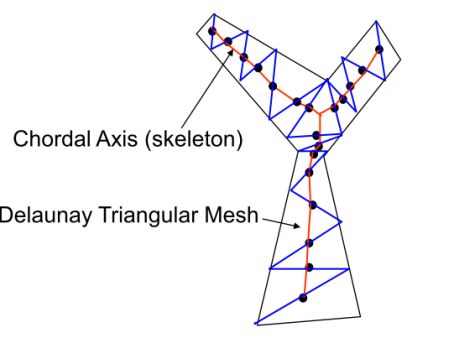
\includegraphics[width=0.4\linewidth]{../Common/images/CAT}} \quad
	\subfloat[CAT Surface for 3D Input]{\label{fig_cat3d}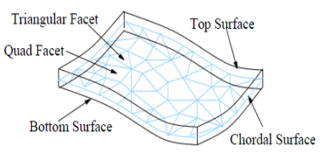
\includegraphics[width=0.4\linewidth]{../Common/images/CAT3D}}
	\caption{Chordal  Axis Transform (Source: Quadros~\cite{QuadrosRoshanOwenBrewerShimada2004} )} %%%%%%%% ADD (\{citeYogeshIITG2014}) LATER
	\label{fig:litsurvey:cat}
	\end{figure}
	
%%\bigskip

CAT was first proposed by Prasad~\cite{Prasad2007} and developed extensively by Quadros~\cite{QuadrosShimadaOwen2004, QuadrosRoshanOwenBrewerShimada2004, Quadros2008}.
Quadros~\cite{QuadrosShimadaOwen2004, Quadros2008, Quadros2000} triangulated the input shape with single layered constrained meshing, classified cells based on positions and had each unit compute their own midsurface patches, which later were joined. With this approach, medials of large, complex parts can be calculated, but the limitation is that getting the uniform, one layered triangulation itself is challenging. Thus, this method is not used for practical, real-life CAE analysis.
	
	
%%Below is the summary of the relevant CAT approaches:
%%
%%\csvreader[longtable=|p{0.17\linewidth}|p{0.09\linewidth}|p{0.12\linewidth}|p{0.2\linewidth}|p{0.17\linewidth}|p{0.17\linewidth}|,
%%    table head=\toprule \bfseries Author & \bfseries Input& \bfseries  Medial& \bfseries  Approach& \bfseries  Advantages& \bfseries  Limitations \\ \midrule \endhead,% \bottomrule \endfoot,
%%  late after last line=\\\bottomrule,
%%  before reading={\catcode`\#=12},after reading={\catcode`\#=6},    
%%    late after line=\\\hline]%
%%{../DocsSources/litsurvey_cat.csv}{Author=\Author, Input=\Input, Method=\Method, Approach=\Approach, Advantages=\Advantages ,Limitations=\Limitations}%
%%{\Author  & \Input&  \Method &\Approach & \Advantages & \Limitations}%
%%
%%\subsubsection{Observations on CAT}
%%
%%\begin{itemize}[noitemsep,topsep=2pt,parsep=2pt,partopsep=2pt]
%%	\item  Similar to MAT, the biggest advantages of CAT is that it can be computed for any thick or thin shape.
%%	\item The major limitation of CAT approach is that mesh has to be generated before the Chordal axis surface can be created. Creating constrained, single layer meshes on complicated solid CAD models are at times difficult.
%%\end{itemize}

\subsection{Generating Midsurface by Thinning Approaches}

\replaced{Thinning approaches}{The algorithms in this category} simulate the grass-fire process~\cite{Harry1967}. In the grass-fire process, when boundary of grass field is set to fire, the fire front successively shrinks the field inwards till it reaches the intersections. \added{In the context of medial computation, the grass-fire process is simulated by making object thinner and thinner in successive iterations} by offsetting its boundary toward its interior until vanishing. %The amount of offset at each step depends on topology and connectivity of the original objects~\cite{KaoJune1999}.

By iteratively offsetting the boundary curves and efficiently identifying the breakpoints, Montanari~\cite{Montanari1969} could locate all the critical points on the medial axis, together with the geometry of the skeleton segments that connect them. Gursoy~\cite{Gursoy1989} extended his work by including circular arcs as boundary elements.

Aichholzer~\cite{Aichholzer1991, Aichholzer2006} was one of the first proponents of a special thinning method called ``Straight Skeletons''. 

%%\bigskip

	\begin{figure} [!h]
		\centering
		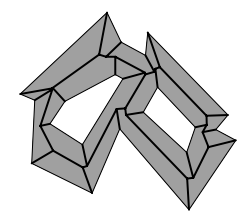
\includegraphics[width=0.4\linewidth]{..//Common/images/Straight}
		\caption{Straight Skeletons (Source: Aichholzer~\cite{Aichholzer1991} )}
		\label{fig:litsurvey:straight}
	\end{figure}
	
%%\bigskip

Figure \ref{fig:litsurvey:straight} shows an example of a Straight Skeleton of a 2D shape. At each vertex angle bisectors are produced. They are used to partition the interiors. The lines joining intersection pins of the bisector forms the medial curve. Although this method can take both, thick and thin shapes, it is restricted to only polygons. Another limitation is that, similar to MAT, it also produces unwanted branches which need to be removed.

%%Below is the summary of the relevant Thinning approaches:
%%
%%\csvreader[longtable=|p{0.17\linewidth}|p{0.1\linewidth}|p{0.12\linewidth}|p{0.2\linewidth}|p{0.17\linewidth}|p{0.17\linewidth}|,
%%    table head=\toprule \bfseries Author & \bfseries Input& \bfseries  Medial& \bfseries  Approach& \bfseries  Advantages& \bfseries  Limitations \\ \midrule \endhead,% \bottomrule \endfoot,
%%  late after last line=\\\bottomrule,
%%  before reading={\catcode`\#=12},after reading={\catcode`\#=6},    
%%    late after line=\\\hline]%
%%{../DocsSources/litsurvey_midsurfthinning.csv}{Author=\Author, Input=\Input, Method=\Method, Approach=\Approach, Advantages=\Advantages ,Limitations=\Limitations}%
%%{\Author  & \Input&  \Method &\Approach & \Advantages & \Limitations}%
%%
%%
%%\subsubsection{Observations on Thinning Approaches}
%%\begin{itemize}[noitemsep,topsep=2pt,parsep=2pt,partopsep=2pt]
%%	\item Thinning approaches are based on split events of the straight line skeleton gives counter-intuitive results if the polygon contains sharp reflex vertices.
%%	\item It generates unwanted branches which need to be removed to arrive at the required midcurve.
%%\end{itemize}

%-------------------------------------------------------------------------------------
\subsection{Generating Midsurface by Parametric Equations Approach}	
\replaced{Parametric}{This} approach takes two parent curves and fits a curve through equidistant points from both the curves~\cite{Elber1999, Fischer1997}. Figure~\ref{fig:litsurvey:parametric} shows two input curves $C_1(u)$ and $C_2(v(u))$ generating midpoint $O(u.v(u0))$. Loci of the $O$s is the midcurve. \added{Same approach can be extended to surfaces as well.}

%%\bigskip

	\begin{figure} [!h]
		\centering
		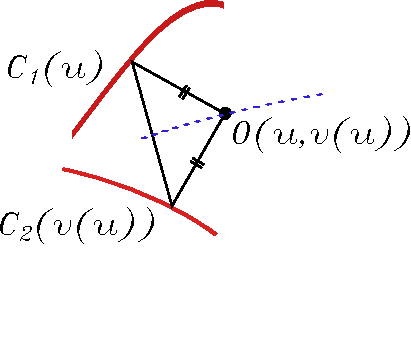
\includegraphics[width=0.4\linewidth]{..//Common/images/MidcurvesDefn}
		\caption{Parametric Midcurve (Source: Fischer~\cite{Fischer1997} )}
		\label{fig:litsurvey:parametric}
	\end{figure}
	
%%\bigskip

In Fischer's~\cite{Fischer1997} parametric approach, sketch profile of features like Extrude, Revolve is extracted. The piecewise linear midpoints  of intersecting pair of matched normals are generated. They are then fitted with the Bspline midcurve. Midcurve is extruded or revolved to generate the midsurface.  This approach gives fairly good results in generating midsurface patches per feature, however, does not elaborate on joining connections between the midsurface patches.

In one of the most recent approaches reported by Zhu et. al~\cite{Zhu2015, Zhu2016}, input surfaces are triangulated, then for each point pair a middle point is computed, which are then fitted with the surface. While this method removes need for post-processing self-intersecting surfaces, it has major drawbacks that it needs surface pairs to be readily available and requires expensive triangulation.

%%Below is the summary of the relevant Parametric Equations  approaches:
%%
%%\csvreader[longtable=|p{0.17\linewidth}|p{0.1\linewidth}|p{0.12\linewidth}|p{0.2\linewidth}|p{0.17\linewidth}|p{0.17\linewidth}|,
%%    table head=\toprule \bfseries Author & \bfseries Input& \bfseries  Medial& \bfseries  Approach& \bfseries  Advantages& \bfseries  Limitations \\ \midrule \endhead,% \bottomrule \endfoot,
%%  late after last line=\\\bottomrule,
%%  before reading={\catcode`\#=12},after reading={\catcode`\#=6},    
%%    late after line=\\\hline]%
%%{../DocsSources/litsurvey_midsurfparam.csv}{Author=\Author, Input=\Input, Method=\Method, Approach=\Approach, Advantages=\Advantages ,Limitations=\Limitations}%
%%{\Author  & \Input&  \Method &\Approach & \Advantages & \Limitations}%
%%
%%\subsubsection{Observations on Parametric Approaches}
%%\begin{itemize}[noitemsep,topsep=2pt,parsep=2pt,partopsep=2pt]
%%	\item The two input curves/surfaces may not be in one-to-one form. In such cases maintaining continuity would a be challenge.
%%	\item Quality of surface generated by these method depends on the sampling done to compute the midpoints.
%%\end{itemize}

Table~\ref{tbl:survey:matcatparamthin} outlines the summary of research contributions in the above mentioned formal approaches.

%%\bigskip

\csvreader[longtable=|p{0.15\linewidth}|p{0.1\linewidth}|p{0.15\linewidth}|p{0.15\linewidth}|p{0.17\linewidth}|p{0.17\linewidth}|,
    table head={\toprule \bfseries Author & \bfseries Input& \bfseries  Medial& \bfseries  Approach& \bfseries  Advantages& \bfseries  Limitations \\ \midrule \endhead \caption{Formal Midsurface Generation Approaches}\label{tbl:survey:matcatparamthin} \endlastfoot},% \bottomrule \endfoot,
  late after last line=\\\bottomrule,
  before reading={\catcode`\#=12},after reading={\catcode`\#=6},    
    late after line=\\\hline]%
{../DocsSources/litsurvey_matcatthinparam.csv}{Author=\Author, Input=\Input, Method=\Method, Approach=\Approach, Advantages=\Advantages ,Limitations=\Limitations}%
{\Author  & \Input&  \Method &\Approach & \Advantages & \Limitations}%


%%\bigskip


\subsection{Observations on Formal Midsurface Generation Approaches}\label{sec:survey:observationsformal}

\todo{[MAKING A NEW (TO BE CONFIRMED) CLASSIFICATION O METHODS INTO FORMAL AND HEURISTIC.Calling MAT, CAT, Thinning and Parametric as Formal methods as they are mathematical and definitive in output. Calling remaining methods like Face Pairing, Feature based, decomposition based as Heuristic as they are non-formal, non-mathematical. Need to discuss and confirm]}


Approaches based on MAT, CAT, Thinning and Parametrization have been in research for decades. All of them, being formal-mathematical, can be applied to wide variety of shapes, and not restricting themselves to only thin shapes. Following are some of the salient observations with regards to these approaches:

\todo{Review comment: Add one liner as differentiator between previous and following approaches. [DONE]}

\begin{itemize}[noitemsep,topsep=2pt,parsep=2pt,partopsep=2pt]
	\item Biggest strength of formal approaches like MAT is that it can be computed for any shape, thick or thin. Being formally defined, the converse or reversal process, meaning ``given a MAT, compute the original shape'', is possible.
	\item Major drawback of MAT, Thinning methods is that it creates unnecessary branches and its shape is smaller than the original corresponding faces.
	\item  MAT based approaches also suffer from robustness problem. A slight change in base geometry forces re-computation of MAT and the results could very well be different from the original.
	\item Although MAT approaches have been around for decades and are fairly mature, its usage in midcurve-midsurface generation is still very complex and difficult to ensure appropriate topology.
	\item The major limitation of CAT approach is that mesh has to be generated before. Creating constrained, single layer meshes on complicated CAD models are, at times, difficult.
	\item Thinning approaches are based on split events of the straight line skeleton giving counter-intuitive results if the polygon contains sharp reflex vertices.
	\item In Parametric approach, the two input curves or surfaces may not be in one-to-one form. In such cases maintaining continuity can be challenging.
	\item Quality of surface generated by parametric approach depends on the sampling done to compute the midpoints.
\end{itemize}

\added{Thus formal approaches to compute midcurve or midsurface have some major limitations, rendering them less useful for the practical scenarios. Following approaches are more heuristic in nature and they are found to have wider applicability in the practical scenarios.} 

\subsection{Generating Midsurface by Face Pairing Approach}
%\subsection{Generating Midsurface by Face Pairing or Midsurface Abstraction Approach}

Midsurface Abstraction (MA) or Face-pairing method was first proposed by Rezayat~\cite{Rezayat1996}. In this approach, face pairs are identified on the thin-wall part's Brep model. It involves casting a ray from a face in the Brep's material direction, to find the opposite face. Such opposite faces form face-pairs. Each face pair generates its own midsurface patch. Connectivity information between respective face-pairs is used to decide which midsurface patches join each other. The midsurface patches are joined, either by trimming or extending them to come to a common location.

%%\bigskip

	\begin{figure} [!h]
		\centering
		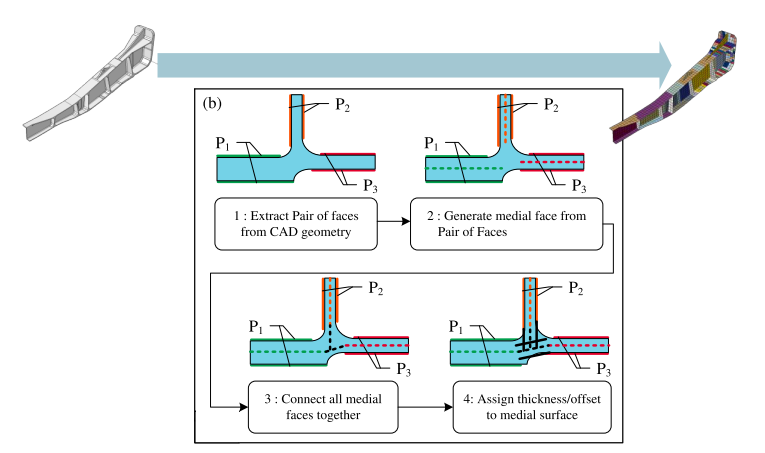
\includegraphics[width=\linewidth]{..//Common/images/manual}
		\caption{Generating Midsurface by Face Pairing (Source: Boussuge~\cite{Boussuge2014})}
		\label{fig:litsurvey:manual}
	\end{figure}
	
%%\bigskip

Figure~\ref{fig:litsurvey:manual} depicts the face pairing approach. Figure~\ref{fig:litsurvey:manual}:1  shows face pairs being detected. In Figure~\ref{fig:litsurvey:manual}:2, midsurface patches are generated for each face pair. In Figure~\ref{fig:litsurvey:manual}:3, patches are extended or trimmed to join at common locations. In Figure~\ref{fig:litsurvey:manual}:4, thickness values are assigned on the midsurface.


\todo{[Removed both the paragraphs and merged info in the first paragraph]}
	
Rezayat claims that the face-pairing approach has benefits over the MAT approach because the resultant geometry is cleaner and requires less post-processing. However the face pairing approach suffers from severe difficulties especially in complex models, such as identifying correct face pairs and joining midsurface patches properly.
	
%Flow of algorithm is as below:
%\begin{itemize}[noitemsep,topsep=2pt,parsep=2pt,partopsep=2pt]
%	\item In the surface pairing step, all the faces excepting the end-caps and of thick region are paired. It involves ray casting from (any) seed face in material direction to find opposite-pair face.
%	\item connectivity between respective faces of pairs is preserved by tagging.
%	\item The paired faces are then interpolated to create mid-surface patches, which may be intersecting. 
%	\item The topological adjacency information (tagged info) is used to trim the patches
%\end{itemize}

%Thus, MA~\cite{Rezayat1996, Fischer1997} involves constructing the 3D mid-surface for a part model by connecting/sewing the mid-surface patches obtained from 'pairs of surfaces'. This requires a 'pairing strategy' that thus far requires human intervention. Connecting various mid-surface patches require 3D Boolean operations. This surface-pairing approach has benefits over MAT approaches because the resultant geometry is cleaner and requires less reconstruction. However the surface pairing approach also has problems because it can be difficult to identify all of the surface pairs.

%%Ramanathan~\cite{Ramanathan2004} states that though the mid-surface has desirable properties as an abstraction of 3D shape, a formal definition of the midsurface is not available. This makes it difficult to develop algorithms for generating the mid-surface of an object. Also, unlike MAT, the mid-surface is not unique for a given object and this adds to the difficulties in realizing the mid-surface. There have been very few efforts reported for the construction of mid-surface.

%The mid-surface abstraction is applied to the entire model simultaneously and no error threshold is defined to select the parts of the model to which abstraction is to be applied. In this approach, small features such as holes are simplified automatically when the mid-surface is generated. Material distribution is effectively represented in this approach by introducing thickening in the direction of the draft and by introducing thinning in the direction of the undercut.

%%Chong et al., who presented an approach to break the Brep model into parts and then applied mid-surface abstraction for simplification for finite element model preparation application\cite{Chong2004}.

S H Lee and D P Sheen~\cite{Sheen2008} proposed Solid Deflection method leveraging face-pair detection and face geometry replacement. Topology was kept intact while bigger of the two faces was offset-ed. Tolerance was increased so as to make them look like connected but they were not. Their work appears to be very limited in the range of input shapes it would handle.
%
%	\begin{figure} [!h]
%		\centering
%		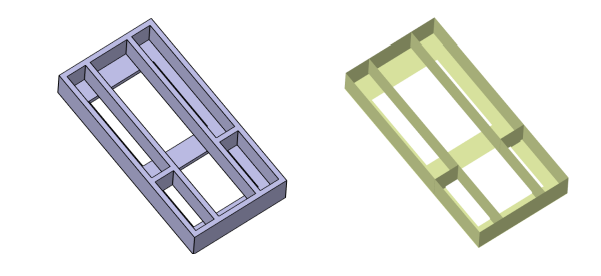
\includegraphics[width=0.6\linewidth]{..//Common/images/SheenMidsurf}
%		\caption{Midsurface Abstraction (Source: Sheen~\cite{Sheen2008} )}
%		\label{fig:litsurvey:sheen}
%	\end{figure}

\todo{Removed the figure. One is good enough}

Sungchan Kim et al.~\cite{Kim2005} developed various approaches for model simplification, mainly focusing on defeaturing aspects, but they also mentioned usage of face-pairing for dimension reduction in case of thin solids. Their approach is simplistic and lacks details on joining of midsurface patches.

%%Below is the summary of the relevant Face Pairing approaches:
%%
%%
%%\csvreader[longtable=|p{0.17\linewidth}|p{0.11\linewidth}|p{0.15\linewidth}|p{0.2\linewidth}|p{0.17\linewidth}|p{0.17\linewidth}|,
%%    table head=\toprule \bfseries Author & \bfseries Input& \bfseries  Method& \bfseries  Approach& \bfseries  Advantages& \bfseries  Limitations \\ \midrule \endhead,% \bottomrule \endfoot,
%%  late after last line=\\\bottomrule,
%%  before reading={\catcode`\#=12},after reading={\catcode`\#=6},    
%%    late after line=\\\hline]%
%%{../DocsSources/litsurvey_midsurfpairing.csv}{Author=\Author, Input=\Input, Method=\Method, Approach=\Approach, Advantages=\Advantages ,Limitations=\Limitations}%
%%{\Author  & \Input&  \Method &\Approach & \Advantages & \Limitations}%

Face-pairing algorithms are implemented in the commercial CAD-CAE applications, mainly rely on intuitiveness and possibility of using manual input. Thus, despite the limitations, these applications are able to generate mid-surfaces for a range of realistic models. Approaches seen so far were based on Brep model. Following section elaborates midsurface generation approaches using feature information.

%A medial surface toolkit is available from TranscenData~\cite{Transcendata2009},
%and the surface-pairing algorithm is implemented in UGS I-DEAS-NX~\cite{SDRC2009}.
%%\subsubsection{Observations on Midsurface-abstraction Approaches}
%%
%%\begin{itemize}[noitemsep,topsep=2pt,parsep=2pt,partopsep=2pt]
%%\item Very popular method amongst commercial implementation as it provides the user the ability to pick appropriate face pairs in case the automatic detection fails. It does not create branches.
%%\item Automatic Face pair detection is error prone in non-trivial situations. Also, connections between patches are missed in complex shapes.
%%\item  Major drawback is that it may not be able to compute midsurface for very complicate parts.
%%\end{itemize}


\subsection{Generating Midsurface by Feature-based Approaches}

In feature based CAD, a model is built step-by-step using features. At each step,  input parameters of the features are used to build tool-bodies. These tool bodies are then boolean-ed with the model built till that step. 

%%\bigskip

	\begin{figure} [!h]
		\centering
		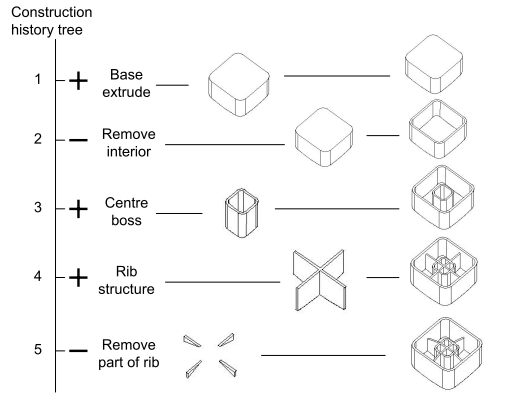
\includegraphics[width=0.75\linewidth]{..//Common/images/stolttree}
		\caption{Construction of CAD Model by Features (Source: Stolt~\cite{Stolt2006} )}
		\label{fig:litsurvey:stolttree}
	\end{figure}

%%\bigskip

Figure~\ref{fig:litsurvey:stolttree} shows Stolt's~\cite{Stolt2006} depiction of construction history, i.e. feature tree of a CAD model. The shapes shown in the middle are the tool bodies, which are boolean-ed (shown as $+$ and $-$) to build the model. In many cases, the tool-bodies are of relatively simple shapes \added{such as extruded or revolved sections,} thus making feature based algorithms simpler and deterministic. There have been a few attempts to use the feature information in the computation of the midsurface. Use of features has not been done extensively in the past because feature specific information was not exposed by the CAD systems, either through file format or through Application Programming Interfaces (APIs). These days, however, most of the widely used CAD modelers provide APIs to expose feature information, giving rise to their usage in CAD algorithms. 

%%%%\bigskip
%%
%%	\begin{figure} [!h]
%%		\centering
%%		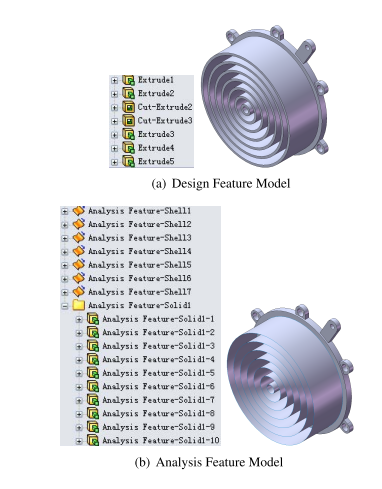
\includegraphics[width=0.6\linewidth]{..//Common/images/CaoMidsurf}
%%		\caption{Midsurface of a Feature based CAD model (Source: Cao~\cite{Cao2009} )}
%%		\label{fig:litsurvey:cao}
%%	\end{figure}
%%
%%%%\bigskip

Stolt~\cite{Stolt2005} worked on features such as ``Pad'', ``Pocket'', extracted sketches and analyzed if there are parallel curves to form mid-segments. These segments are used for extrusion with same parameters as the original feature.

%%\bigskip

	\begin{figure} [!h]
		\centering
		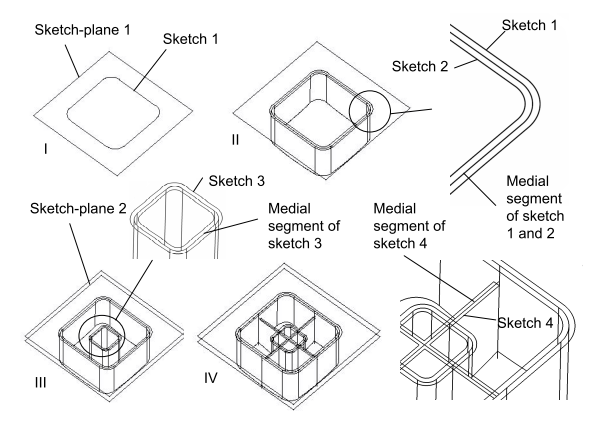
\includegraphics[width=0.75\linewidth]{..//Common/images/stoltmids}
		\caption{Construction of Feature-based Midsurface (Source: Stolt~\cite{Stolt2006} )}
		\label{fig:litsurvey:stoltmids}
	\end{figure}

%%\bigskip

Figure~\ref{fig:litsurvey:stoltmids} shows the process of building feature based midsurface proposed by Stolt ~\cite{Stolt2006}. Figure~\ref{fig:litsurvey:stoltmids}:I shows the first feature's sketch. Figure~\ref{fig:litsurvey:stoltmids}:II shows the first feature, along with its midsurface computed from the medial segment of the first sketch. Similarly Figure~\ref{fig:litsurvey:stoltmids}III and IV show, features being added along with their midsurface.

Robinson et al.~\cite{Robinson2007} while working on mixed-dimensional model for aerospace structures utilized information in CAD feature tree to locate sketches and then features built on top of it like Sweep, Revolve. The work appears to be limited due to processing of a small set of singular features only and no consideration seems to be given to joining process.

These approaches are comparatively less in number and restrict themselves to midsurface patches creation. They do not leverage feature information effectively in setting up appropriate connections between patches.

%%As Brep is still the most widely used format, some apparhches do Feature recognition to extract features and then apply their midurface generation aleotithms.
%% 
%%Figure~\ref{fig:litsurvey:cao} shows how Cao~\cite{Cao2009}~\cite{Cao2011} decomposed the final Brep and recognized additive remnant swept primitives for which midsurface patches were computed either by sweeping corresponding midcurve or offsetting one of the faces or by interpolating the faces. But there no details mentioned about joining logic for the patches.
%%
%%Boussuge et al. ~\cite{Boussuge2013,Boussuge2013a} split the Brep into protrusion features and then idealized each to midsurface. The joining logic presented in this work was very restricted to 3 interaction types and also the features recognized were only positive protrusions.

\todo{[REMOVED FIGURE FROM HERE AND LET IT BE WHERE IT IS MOST APPROPRIATE]}


%%Below is the summary of the relevant feature based midsurface approaches:
%%
%%\csvreader[longtable=|p{0.17\linewidth}|p{0.11\linewidth}|p{0.15\linewidth}|p{0.2\linewidth}|p{0.17\linewidth}|p{0.17\linewidth}|,
%%    table head=\toprule \bfseries Author & \bfseries Input& \bfseries  Medial& \bfseries  Approach& \bfseries  Advantages& \bfseries  Limitations \\ \midrule \endhead,% \bottomrule \endfoot,
%%  late after last line=\\\bottomrule,
%%  before reading={\catcode`\#=12},after reading={\catcode`\#=6},    
%%    late after line=\\\hline]%
%%{../DocsSources/litsurvey_midsurffbd.csv}{Author=\Author, Input=\Input, Method=\Method, Approach=\Approach, Advantages=\Advantages ,Limitations=\Limitations}%
%%{\Author  & \Input&  \Method &\Approach & \Advantages & \Limitations}%
%%
%%
%%\subsubsection{Observations on Feature based Midsurface Approaches}
%%
%%\begin{itemize}[noitemsep,topsep=2pt,parsep=2pt,partopsep=2pt]
%%\item Feature based approaches bring definitiveness in model simplification which in turn helps midsurface idealization
%%\item Feature information has not been extensively used for variety of reasons such as access-restrictions on the proprietary feature information, unsuitable non-manifold structure, as well as the impracticality to include CAE structures in CAD software.
%%\item Most of the approaches restrict themselves to midsurface patches creation and do not leverage feature boolean information in setting up appropriate connections between patches.
%%\end{itemize}


\subsection{Generating Midsurface by Decomposition Based Approaches}

Decomposition is a process of partitioning given shape into non overlapping sub-shapes. It can be applied on both, 2D and 3D CAD shapes. Decomposed sub-shapes compute the medial object. If 2D sketch profiles is the input then, midcurves are computed and if 3D Brep solid is the input then midsurface is computed. 


%%\bigskip

	\begin{figure} [!h]
		\centering
		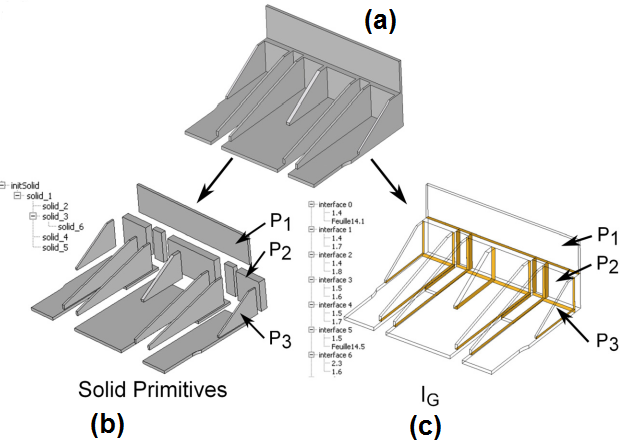
\includegraphics[width=0.75\linewidth]{..//Common/images/boussugedecomp}
		\caption{Generating Midsurface by Decomposition (Source: Boussuge~\cite{Boussuge2013a} )}
		\label{fig:litsurvey:boussugedecomp}
	\end{figure}

%%\bigskip

Figure~\ref{fig:litsurvey:boussugedecomp} depicts Boussuge's~\cite{Boussuge2013a} approach of midsurface by decomposition.
Figure~\ref{fig:litsurvey:boussugedecomp}a shows the input Brep solid CAD model. Figure~\ref{fig:litsurvey:boussugedecomp}b shows its decomposition into sub-shapes, called ``solid primitives''. Figure~\ref{fig:litsurvey:boussugedecomp}c shows midsurface computed for each solid primitive.
\todo{[MOVED PARAGRAPHS OF POLYGON DECOMPOSITION AND MIDCURVE CREATION TO THAT CHAPTER. MIDCURVE COULD HAVE BEEN RETAINED HERE, BUT THEN WITHOUT POLY DECOMP IT WAS NOT MAKING SENSE.]}

%\subsubsection{Generating Midcurve by 2D Decomposition}

%%Midcurve by 2D decomposition methods are based on Divide-and-Rule policy. The 2D profile is subdivided into simpler sub-shapes for which medial can be computed readily. Midcurves of all such sub-shapes are merged to get the final well-connected midcurve.
%%
%%Keil~\cite{Keil94} presented an approach based on Convex partitioning. It finds all possible ways to remove reflexivity of these vertices and then takes the one that requires fewest diagonals. Lien et. al.~\cite{Lien2004} decomposed polygons 'approximately' based on iterative removal of the most significant non-convex feature. 
%%
%%Bayazit~\cite{Bayazit} presented a polygon decomposition method based on Concave (Reflex) angle partitioning. Although the output was far better than if usual meshing had been employed, the drawback was it left out some corner cases giving more than necessary divisions.
%%
%%Below is the summary of the relevant profile decomposition approaches:
%%
%%\csvreader[longtable=|p{0.17\linewidth}|p{0.11\linewidth}|p{0.15\linewidth}|p{0.2\linewidth}|p{0.17\linewidth}|p{0.17\linewidth}|,
%%    table head=\toprule \bfseries Author & \bfseries Input& \bfseries  Method & \bfseries  Approach& \bfseries  Advantages& \bfseries  Limitations \\ \midrule \endhead,% \bottomrule \endfoot,
%%  late after last line=\\\bottomrule,
%%  before reading={\catcode`\#=12},after reading={\catcode`\#=6},    
%%    late after line=\\\hline]%
%%{../DocsSources/litsurvey_polydecomp.csv}{Author=\Author, Input=\Input, Method=\Method, Approach=\Approach, Advantages=\Advantages ,Limitations=\Limitations}%
%%{\Author  & \Input&  \Method &\Approach & \Advantages & \Limitations}%
%%
%% Choi~\cite{Choi1997} subdivided the planar region with holes into smaller simply connected planar sub regions that overlap only at the joints where subdivision occurs. Approximated medials based on Bezier-Bernstein curves are computed for individual sub-regions. Decomposition of planar shapes  into regular (non-intersecting) and singular (intersecting regions) and its application to skeletonization has been widely researched~\cite{Rocha99} as well.
%% 
%% Rocha~\cite{Rocha98}~\cite{Rocha99} presented skeletonization approach for images which primarily worked on vertices. Sub-shapes computed mid-segments which were joined at the connections. Although this approach could address many shapes, it lacked comprehensive coverage and did not do very well for simple joints like T and L
%%
%%Bag~\cite{Bag2011} computed mid-segments for character image which preserve the local characteristics.
%% 
%% Below is the summary of the relevant midcurve computation approaches:
%% 
%%\csvreader[longtable=|p{0.17\linewidth}|p{0.11\linewidth}|p{0.2\linewidth}|p{0.2\linewidth}|p{0.17\linewidth}|p{0.17\linewidth}|,
%%    table head=\toprule \bfseries Author & \bfseries Input& \bfseries  Medial& \bfseries  Approach& \bfseries  Advantages& \bfseries  Limitations \\ \midrule \endhead,% \bottomrule \endfoot,
%%  late after last line=\\\bottomrule,
%%  before reading={\catcode`\#=12},after reading={\catcode`\#=6},    
%%    late after line=\\\hline]%
%%{../DocsSources/litsurvey_midcurvedecomp2d.csv}{Author=\Author, Input=\Input, Method=\Method, Approach=\Approach, Advantages=\Advantages ,Limitations=\Limitations}%
%%{\Author  & \Input&  \Method &\Approach & \Advantages & \Limitations}%
%%
%%\subsubsection{Observations on Midcurve by 2D Decomposition Approaches}
%%
%%\begin{itemize}[noitemsep,topsep=2pt,parsep=2pt,partopsep=2pt]
%%	\item Polygon decomposition rules depend on the application context, accuracy, characteristics  and aspect ratio of the sub-polygons. In CAE, meshing is one of the widely used decomposition methods. Approiach used in this work aims at minimum partitioning to result into primitive shaped sub-polygons.
%%	\item Midcurve generation depends on the quality of the sub-polygons generated in the decomposition. Non-primitive, skewed shapes result in ill-midcurves.
%%\end{itemize}


%\subsubsection{Generating Midsurface by Cellular Decomposition}

\added{The sub-shapes generated by decomposition are called as ``Cells''. Cells not only simplify the geometries to work with but also introduce possibility of parallelization. With these advantages, researchers have used decomposition extensively in CAD (as voxels), CAM (machining pockets), CAE (meshing), etc.}

%%The present research leverages decomposition for devising generic midsurface computations algorithm. One of the primary reasons for gaps in the midsurface results is due to ill-recording  of feature interaction in the input shape. Thus, same interaction could not get replicated on the midsurface patches.  To address issues related to feature interactions, this research leverages feature based CAD model represented as a set of decomposed cells. 

\todo{[MOVED CELLULAR DECOMPOSITION SPECIFIC SURVEY TO THAT CHAPTER. KEEPING APPROACHES HAVING MIDSURFACE ONLY]}

%%Following subsections present state-of-the-art in Cellular Decomposition, solid model based decomposition, feature based cellular topology and midsurface based on cellular decomposition.
%%
%%\todo{Including few of the cellular decomposition methods that have not been used for midsurface, because, even those methods are useful reference in the decomposition we leveraged}
%%
%%Woo~\cite{Woo2003} found that in typical Cell Decomposition each of the faces having a concave edge is extended such that it interests the whole model, creating cells. As this would generate a large number of unnecessary cells, concept of `maximal volume' came (Figure~\ref{fig:litsurvey:maxcd}), which collects some of the cells, based on certain criteria, to be merged together, thus reducing the number with a few modifications. 
%% 
%%\begin{figure}[!h]
%%\centering     %%% not \center
%%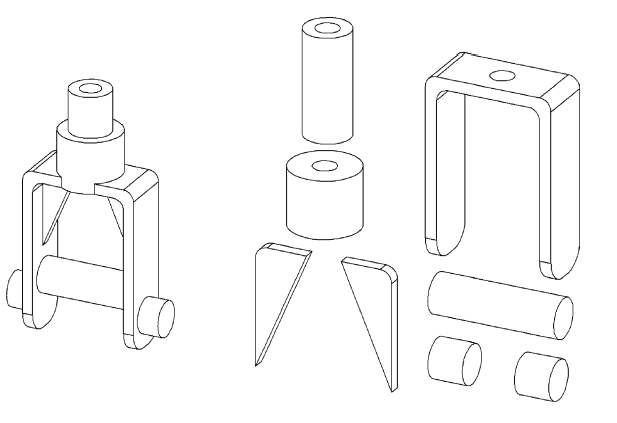
\includegraphics[width=0.5\linewidth,valign=t]{../Common/images/maximalvolume}
%%\caption{Maximal Cellular Decomposition (Source : Woo~\cite{Woo2003})}
%%\label{fig:litsurvey:maxcd}
%%\end{figure}
%% 
%%Bih-Yaw Shih~\cite{Shih1996} presented an automated swept volume detection and decomposition algorithm. This approach was computationally intensives for complex model. 
%%
%%Yong Lu~\cite{LuGadhTautges2001} reported the work on shape recognition and volume decomposition to automatically decompose a CAD model into hex meshable volumes. 
%%
%%Yoonhwan Woo~\cite{Woo2002}~\cite{Woo2003}~\cite{Woo2003a}~\cite{Woo2006}~\cite{Woo2009}  did extensive work in fast and maximal cellular decomposition. His method was superior to other prevalent method but was restricted to analytical surface shapes.
%%
%%%Quite a few attempts to compute the midsurface using cellular decomposition are found in the literature~\cite{Chong2004, Cao2009,Cao2011,Woo2013}.
%%
%% Below is the summary of the relevant Cellular Decomposition approaches:
%% 
%%\csvreader[longtable=|p{0.17\linewidth}|p{0.11\linewidth}|p{0.2\linewidth}|p{0.2\linewidth}|p{0.17\linewidth}|p{0.17\linewidth}|,
%%    table head=\toprule \bfseries Author & \bfseries Input& \bfseries  Method & \bfseries  Approach& \bfseries  Advantages& \bfseries  Limitations \\ \midrule \endhead,% \bottomrule \endfoot,
%%  late after last line=\\\bottomrule,
%%  before reading={\catcode`\#=12},after reading={\catcode`\#=6},    
%%    late after line=\\\hline]%
%%{../DocsSources/litsurvey_celldecomp.csv}{Author=\Author, Input=\Input, Method=\Method, Approach=\Approach, Advantages=\Advantages ,Limitations=\Limitations}%
%%{\Author  & \Input&  \Method &\Approach & \Advantages & \Limitations}%

%%Cellular decomposition, in the context of the current research, is the division of a feature based CAD model into non-volumetrically overlapping, but surface-overlapping sub-solids (called ``cells'').  Research in  cellular decomposition, especially for Computer-aided Manufacturing (CAM) and CAE has been going on for decades. Feature based cellular decomposition, which deals with either decomposition of features, or feature-recognition after decomposition,  has also been  researched extensively~\cite{Bidarra1993, BidarraKrakerBronsvoort1998, Woo2003, JaeLee2004, Treeck, Boussuge2013a, Wu2014, Woo2014}. There have been a few attempts to compute a midsurface using cellular-decomposition as well~\cite{Chong2004, Woo2013, Boussuge2013, Zhu2015}
%% 
%%\csvreader[longtable=|p{0.17\linewidth}|p{0.11\linewidth}|p{0.2\linewidth}|p{0.2\linewidth}|p{0.17\linewidth}|p{0.17\linewidth}|,
%%    table head=\toprule \bfseries Author & \bfseries Input& \bfseries  Method & \bfseries  Approach& \bfseries  Advantages& \bfseries  Limitations \\ \midrule \endhead,% \bottomrule \endfoot,
%%  late after last line=\\\bottomrule,
%%  before reading={\catcode`\#=12},after reading={\catcode`\#=6},    
%%    late after line=\\\hline]%
%%{../DocsSources/litsurvey_featurecells.csv}{Author=\Author, Input=\Input, Method=\Method, Approach=\Approach, Advantages=\Advantages ,Limitations=\Limitations}%
%%{\Author  & \Input&  \Method &\Approach & \Advantages & \Limitations}%

%\subsubsection{Generating Midsurface by Feature based Cellular Decomposition Approaches}

%Feature based Cellular data model has been research and its usage in various downstream applications has been studied. Kernels like ACIS provide cellular topology which can be enhanced to have owner feature information.  
Quite a few attempts to compute the midsurface using cellular decomposition are found in the literature~\cite{Chong2004, Cao2009,Cao2011,Woo2013}. 

%%\bigskip

%
%\begin{figure}[!h]
%\centering     %%% not \center
%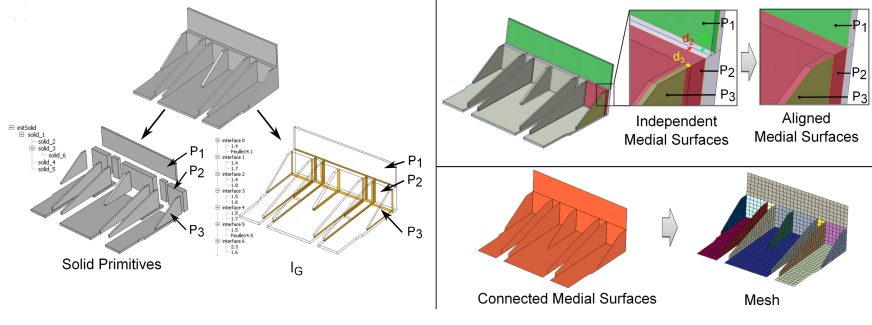
\includegraphics[width=0.85\linewidth,valign=t]{../Common/images/boussugemidsurf}
%\caption{Decomposition, Protrusions, Midsurfaces (Source : Boussuge~\cite{Boussuge2013a})}
%\label{fig:litsurvey:boussuge}
%\end{figure}


\begin{figure}[!h]
\centering     %%% not \center
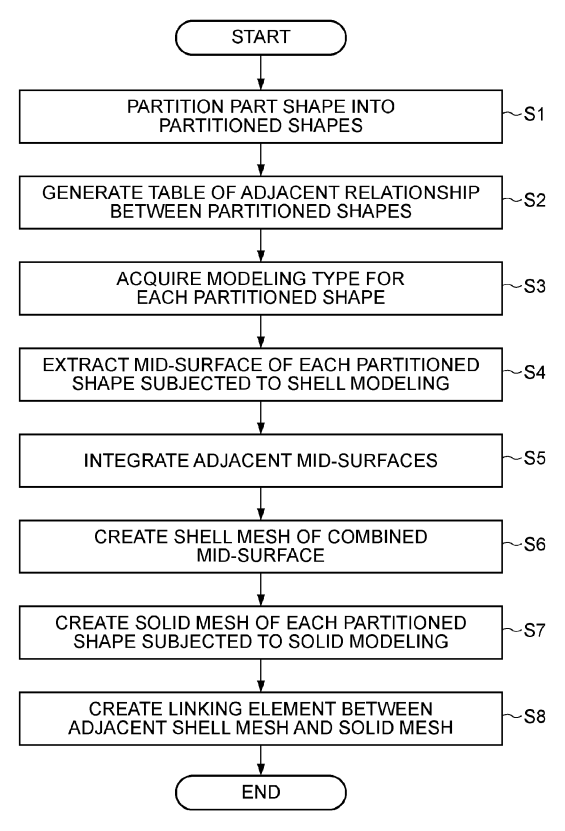
\includegraphics[width=0.45\linewidth,valign=t]{../Common/images/Kageura}
\caption{Generating Midsurface by Partition Approach (Source : Kageura~\cite{Kageura2009})}
\label{fig:litsurvey:Kageura}
\end{figure}

%%\bigskip

Chong et al.~\cite{Chong2004} split the Brep model into sub-volumes which, in turn, extracted their own midsurface patches.

Kageura~\cite{Kageura2009} has filed US Patent 2009/0271156 A1 in which, as shown in Figure~\ref{fig:litsurvey:Kageura},  an input shape is partitioned first, adjacency information is generated, midsurface patches are extracted and combined.

Cao~\cite{Cao2009, Cao2011} decomposed the final Brep model and recognized additive remnant swept primitives, got their sketches, computed midcurves for edge-pairs and created midsurface patches but the joining logic was not much elaborated. 

Boussuge et al. ~\cite{Boussuge2013,Boussuge2013a}  split the Brep model at concave edges, recognized (only) positive  protrusion features in the sub-volumes and then idealized each to a midsurface with a joining logic restricted to only a couple of hard-coded interaction types. Figure~\ref{fig:litsurvey:boussugedecomp} shows how a model is split into solid primitives, midsurface patches are generated and they are joined at the interfaces $I_G$s.

Woo~\cite{Woo2013} used his maximal volume technique (\cite{Woo2006, Woo2009} ) and computed midsurface for each sub-volume using face-pair technique. It worked only for analytical surfaces and parallel face pairs

%% Below is the summary of the relevant Feature based Cellular Decomposition Approaches:
%% 
%%\csvreader[longtable=|p{0.17\linewidth}|p{0.11\linewidth}|p{0.2\linewidth}|p{0.2\linewidth}|p{0.17\linewidth}|p{0.19\linewidth}|,
%%    table head=\toprule \bfseries Author & \bfseries Input& \bfseries  Medial& \bfseries  Approach& \bfseries  Advantages& \bfseries  Limitations \\ \midrule \endhead,% \bottomrule \endfoot,
%%  late after last line=\\\bottomrule,
%%  before reading={\catcode`\#=12},after reading={\catcode`\#=6},    
%%    late after line=\\\hline]%
%%{../DocsSources/litsurvey_midsurfdecomp3d.csv}{Author=\Author, Input=\Input, Method=\Method, Approach=\Approach, Advantages=\Advantages ,Limitations=\Limitations}%
%%{\Author  & \Input&  \Method &\Approach & \Advantages & \Limitations}%

 Table~\ref{tbl:survey:midsheuristic} presents a summary of some of the important heuristic midsurface generation Approaches:
 
 
%%\bigskip

\csvreader[longtable=|p{0.15\linewidth}|p{0.1\linewidth}|p{0.15\linewidth}|p{0.15\linewidth}|p{0.17\linewidth}|p{0.17\linewidth}|,
%    table head=\toprule \bfseries Author & \bfseries Input& \bfseries  Medial& \bfseries  Approach& \bfseries  Advantages& \bfseries  Limitations \\ \midrule \endhead,% \bottomrule \endfoot,
    table head={\toprule \bfseries Author & \bfseries Input& \bfseries  Medial& \bfseries  Approach& \bfseries  Advantages& \bfseries  Limitations \\ \midrule \endhead \caption{Heuristic Midsurface Generation Approaches}\label{tbl:survey:midsheuristic} \endlastfoot},% \bottomrule \endfoot,
     late after last line=\\\bottomrule,
  before reading={\catcode`\#=12},after reading={\catcode`\#=6},    
    late after line=\\\hline]%
{../DocsSources/litsurvey_heuristics.csv}{Author=\Author, Input=\Input, Method=\Method, Approach=\Approach, Advantages=\Advantages ,Limitations=\Limitations}%
{\Author  & \Input&  \Method &\Approach & \Advantages & \Limitations}%


%%\bigskip

\subsection{Observations on Heuristic Midsurface Generation Approaches}

Extensive research has been done on the heuristic methods for computing midsurface, such as midsurface abstraction (face pairing), feature based, cellular decomposition based, etc. These are more widely used in commercial applications, compared to the formal approaches such as MAT, CAT, etc. Even with better  demand, the heuristic methods are limited, especially in case of complex models. Following are salient observations on heuristic methods:

\begin{itemize}[noitemsep,topsep=2pt,parsep=2pt,partopsep=2pt]
\item Face pairing is widely used approach amongst the commercial CAD-CAE applications, as it provides the user the ability to pick appropriate face pairs in case the automatic detection fails. 
\item Automatic Face pair detection is error prone for complex CAD models as input. Joining midsurface patches also does not work robustly for them. Due to these problems, Face pairing suffers from limitations such as extensive use of hard-coded rules for detecting edge or face pairs, support for limited types of geometries, limited range of connections, etc.
\item Midsurface by cellular decomposition approach is not used widely. Cellular decomposition can result in large number of cells, needing quite a few boolean operations, making it ineffective and unstable. Choosing correct splitting logic, maximal volume rules should help make the process optimized and robust.
\item Feature based midsurface computation approaches bring definitiveness in computation of midsurface, due to lesser use of heuristics.
\item Feature information has not been extensively used for computation of midsurface due to its inaccessibility so far. 
\item Most current feature based midsurface computation approaches restrict themselves to midsurface patches creation and do not leverage feature boolean information in setting up appropriate connections between patches.
 \end{itemize}

Overall, both formal and heuristic approaches present strengths and limitations in different aspects of computing midsurface. Out of them, use of defeaturing, leveraging feature information and decomposition appear promising in computation of a quality midsurface. 

The quality of midsurface is validated by various techniques, primarily to detect failures such as gaps, overlaps, etc.
%The present research work attempts to address these limitations by leveraging feature-based, decomposition approaches along with use of new concepts such as generalization, feature based decomposition, etc.
Following section elaborates state of the art for techniques used in validating the quality of the output midsurface.

\deleted{So, this research does not need to utilize the maximal (\cite{Woo2002}) volume strategies that have to be employed due to a large number of cells computed during the global intersections. This research expects that the FBCD should generate the part  decomposed in such a way that each cell represents a correctly assigned owning-feature.More details about methods for computing medial objects can be found in the survey paper by Kulkarni et. al~\cite{Yogesh2010}.}
 
\section{Validation Approaches for Generated Midsurfaces} \label{sec:litsurvey:validation}

Even after huge demand, extensive research and wide availability in the commercial CAD-CAE applications, quality of the midsurface computed is still a concern. Validating the output midsurface is therefore a critical step in assessing the quality, after which corrective actions can be taken.

Midsurface is expected to express the contiguous flow of the input solid's shape~\cite{Rezayat1996}. So, to be truly effective, the output midsurface needs to mimic the input thin-walled solid model, in both, geometrical and topological sense. Geometrically, the shape of the midsurface should be such that it lies in the middle (at half the thickness) of the thin-walled solid model. Topologically, the connectivity between the midsurface patches should be similar to that of their corresponding face pairs in the input thin-walled solid model. 

\deleted{It is tedious to manually inspect and validate it, especially for the complex models. The present system performs such a validation in an automated way and uses Hausdorff's distance measure to verify geometric correctness. However, as a necessary and sufficient validation, the system also carries out topological validation to verify the connectivity as well as missing surfaces or gaps.}

Thus, there are primarily two approaches to validate the output midsurfaces, namely ``geometric'' and ``topological'' ~\cite{Lockett2008} as explained below:

\begin{itemize}[noitemsep,topsep=2pt,parsep=2pt,partopsep=2pt]
\item \textbf{Geometric Validation of Midsurface}: Validates if the output midsurface lies midway of the input solid model. Lockett~\cite{Lockett2008} proposed geometric similarity index based on Hausdorff distance which provides a measure of the maximum dissimilarity between the midsurface and its associated input solid model.
\item \textbf{Topological Validation of Midsurface}:
\deleted{Use of topology for assessing the quality of midsurface is not widespread and t}
Validates if the output midsurface has similar topological connectivity as present in the input solid model. Lockett~\cite{Lockett2008} predicted topological entities of midsurface based on the topological entities of the input solid model and then used topological variants for checking the validity of the midsurface. \deleted{For geometric validation, they used the Hausdorff distance between a midsurface and its corresponding principal faces (pairs).} The main limitation of their approach is the use of geometric criteria, such as closest distance proximity or angle between faces, in the topological validations, which is contrary to the concept of topology.
\end{itemize}

\deleted{Apart from CAE, skeletal structures such as midsurface are used in CAD model comparison solutions such as shape-based retrieval, similarity assessment and difference identification ~\cite{Antoine2014}. Skeletal graph matching is one of the prominent techniques~\cite{Iyer2005} for similarity assessment. A topologically valid midsurface represents sub-shape connectivities better and thus acts as more effective shape-signature in the model comparison.}

\todo{[DROPPED THE TABLE AND OBSERVATIONS]}

%%
%% Below is the summary of the relevant Topological Invariants and Similarity assessment Approaches:
%% 
%%\csvreader[longtable=|p{0.15\linewidth}|p{0.15\linewidth}|p{0.2\linewidth}|p{0.2\linewidth}|p{0.17\linewidth}|p{0.19\linewidth}|,
%%    		table head=\toprule \bfseries Author & \bfseries Input& \bfseries  Method & \bfseries  Approach& \bfseries  Advantages& \bfseries  Limitations \\ \midrule \endhead,
%%    		late after last line=\\\bottomrule,
%%    		before reading={\catcode`\#=12},after reading={\catcode`\#=6},
%%    		late after line=\\\hline]%
%%    		{../DocsSources/litsurvey_validation.csv}
%%    		{Author=\Author, Input=\Input, Method=\Method, Approach=\Approach, Advantages=\Advantages ,Limitations=\Limitations}%
%%    		{\Author  & \Input&  \Method &\Approach & \Advantages & \Limitations}%

%%\subsection{Observations on Midsurface Validation Approaches}
%%
%%\begin{itemize}[noitemsep,topsep=2pt,parsep=2pt,partopsep=2pt]
%%\item Apart from CAE, skeletal structures such as midsurface are used in CAD model comparison solutions such as shape-based retrieval, similarity assessment and difference identification ~\cite{Antoine2014}. 
%%\item Skeletal graph matching is one of the prominent approaches~\cite{Iyer2005} for similarity assessment. 
%%\item A topologically valid midsurface represents sub-shape connectivities better and thus acts as more effective shape-signature in the model comparison.
%%
%%
%%\end{itemize}

Although geometric approaches of validating the output midsurface are widely used, they are tedious to execute. Topological approaches are not very common and are not yet fully developed to be used practically. 

\section{Midsurface Generation Capabilities of Commercial CAD-CAE Systems}\label{sec:litsurvey:commercial}

Commercial CAD-CAE systems are in use for decades. Both systems got developed separately and are like islands of automation. The corresponding commercial systems have to transfer model data amongst themselves only through neutral file formats. Thats the reason, most of the CAD-CAE approaches are based on Brep model populated by neutral file formats, such as STEP and IGES.  Data interoperability through neutral formats is susceptible to data loss. Thus most of the data coming to preprocessing from CAD systems, has to be cleaned and healed first. But, now a days, with better CAD-CAE systems integrations, native data and in some cases even feature information is made available to CAE systems. With richer information, some of the CAD-CAE systems have improved preprocessing functionalities like defeaturing and midsurface generation. 

CAD kernels like ACIS\textsuperscript{\textregistered}, modelers like Autodesk Fusion\textsuperscript{\textregistered} and CAE packages like Altair's Hypermesh\textsuperscript{\textregistered}, Ansys\textsuperscript{\textregistered}, MSc Nastran\textsuperscript{\textregistered}, etc. do provide defeaturing capabilities mainly for CAE analysis\replaced{ that are primarily}{, but are mostly simplistic and } size-based in nature. 

Midsurface functionality is widely available in CAD-CAE systems like Autodesk Inventor\textsuperscript{\textregistered}, Parametric's Creo,  Altair's Hypermesh\textsuperscript{\textregistered}, Ansys\textsuperscript{\textregistered}, MSc Nastran\textsuperscript{\textregistered}, etc. It is observed that quality of midsurface in CAD systems is relatively lower than the CAE systems. But overall, automatic midsurface generation capabilities do not seem to be robust and meaningful for practical usages, especially for complex parts. Manual intervention and post-processing is used to correct the problems of the output midsurface.

\todo{[SHOULD I ADD SCHEMATIC DIAGRAMS SHOWING ERRORS?]}

%%\bigskip

\def \myfigcommcolumnwidth{0.85}

\begin{figure}[h!]
\centering     %%% not \center
\subfloat[Input Thin-walled Solid Model]{\label{fig_mmodel}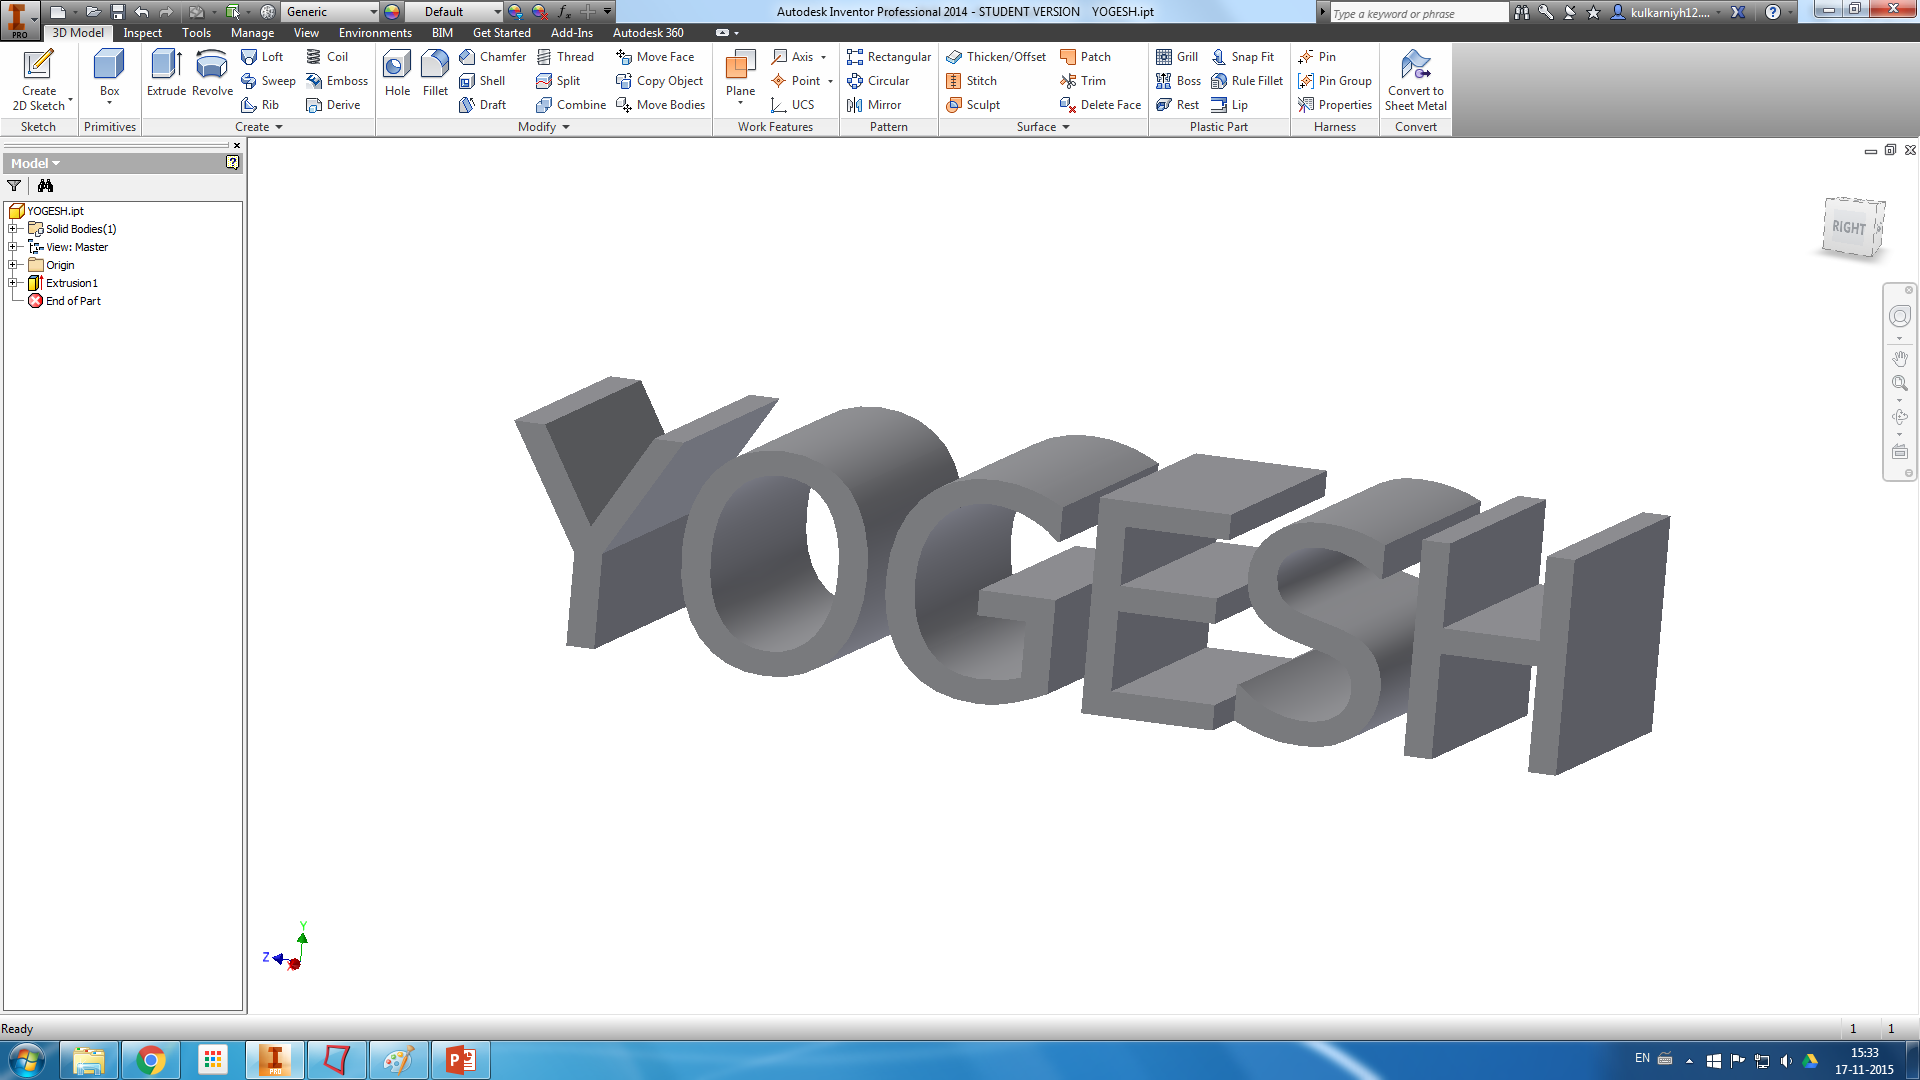
\includegraphics[width=\myfigcommcolumnwidth\linewidth]{../Common/images/Yogesh_Inv}} \quad
\subfloat[Output Midsurface of a CAD System]{\label{fig_mcad}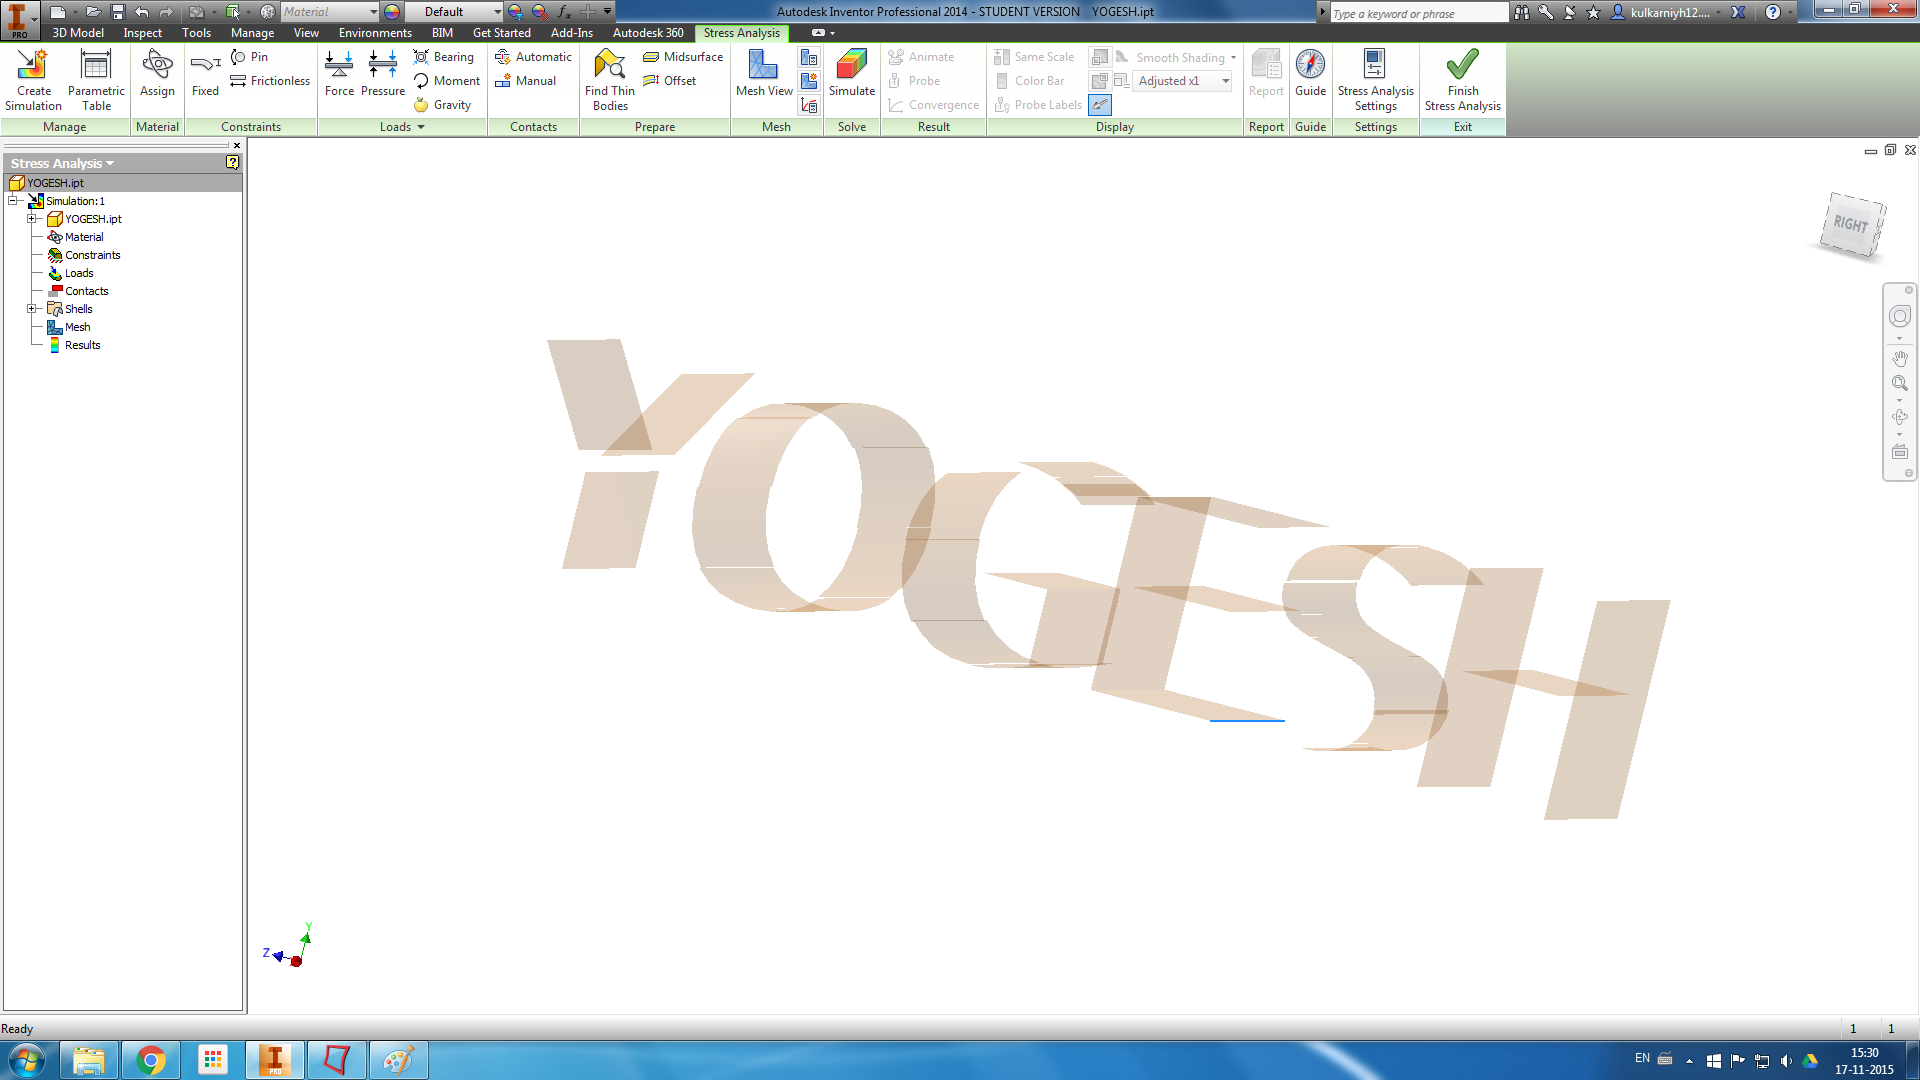
\includegraphics[width=\myfigcommcolumnwidth\linewidth]{../Common/images/Yogesh_InvMids}} \quad
\subfloat[Output Midsurface of a CAE System]{\label{fig_mcae}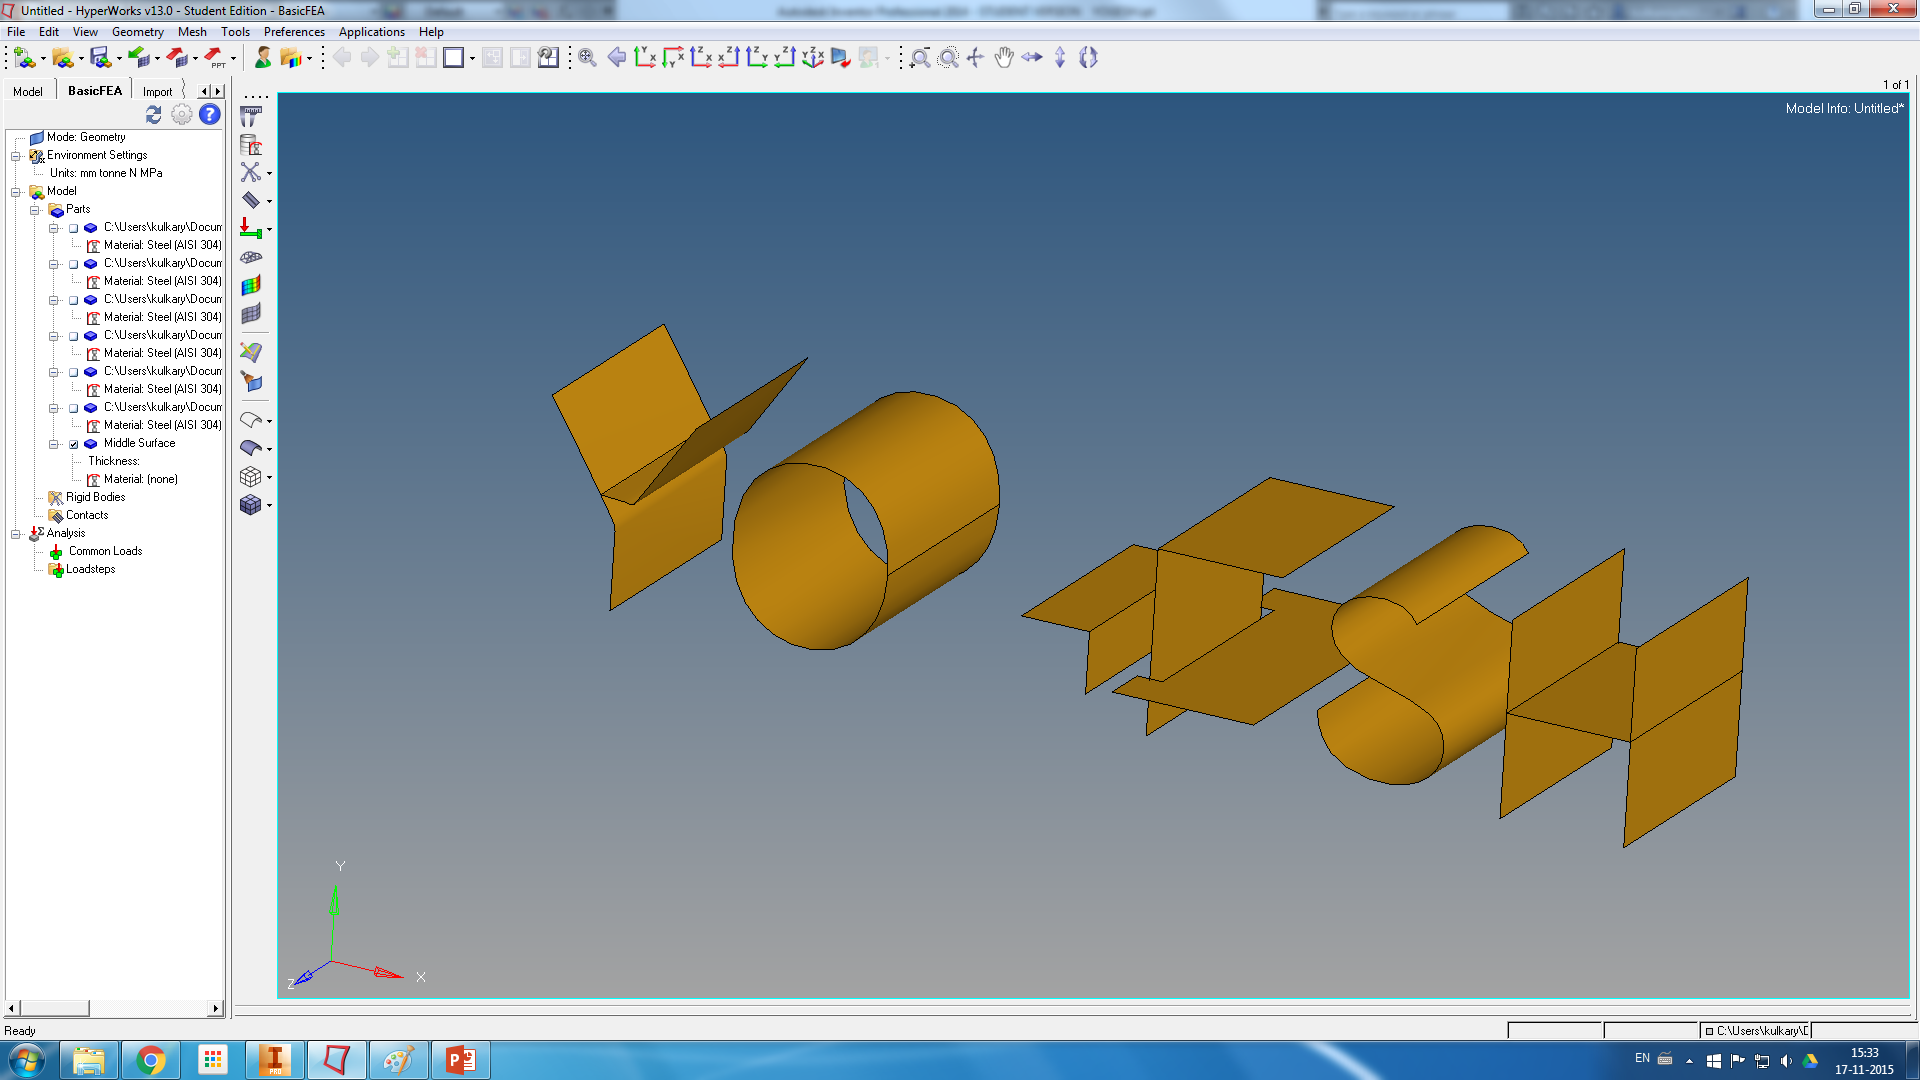
\includegraphics[width=\myfigcommcolumnwidth\linewidth]{../Common/images/Yogesh_HM_notOK}} 
\caption{Midsurfaces Generated by Commercial CAD and CAE Systems}
  \label{fig_comm}
\end{figure}


%%\bigskip

\added{Figure~\ref{fig_comm}a shows the input CAD solid model, having English alphabets shapes. These shapes are chosen for benchmarking, as it is easier to imagine their corresponding midsurfaces. The resultant midsurface is expected to look like those alphabets but in the surface form. Figure ~\ref{fig_comm}b shows midsurface output generated by a popular CAD system, whereas Figure ~\ref{fig_comm}c shows midsurface output by a widely used CAE system. Both CAD and CAE midsurface outputs show many errors, such as missing surfaces, gaps, not-lying-midway, etc.}

From the above results it is evident that there is still an ample scope for improvement in devising a robust and automated method for computing a quality midsurface.

Another detailed survey was done by conducting technical discussions with CAD-CAE experts, academicians related to various aspects of midsurface generation.  This was essentially aimed at understanding industry practices, issues etc.  Findings from theses discussions are provided in Appendix~\ref{appendix:survey}.


%\section{Observations from Survey Questionnaire}\label{sec:litsurvey:questions}

%Below is such list of understandings :
%
%\begin{itemize}[noitemsep,topsep=2pt,parsep=2pt,partopsep=2pt]
%\item 
%\end{itemize}
%
%.
%Many a times, due to complexity in recognizing forms, and due to complex interactions between them, Midsurface of the part does not follow its form and is not fully connected~\cite{Sheen2008}. Solution could be, to create Midsurface while building the model itself. 

\section{Observations from Literature Survey}\label{sec:litsurvey:summary}

%%\todo{These are the overall observations}

After analyzing various reported approaches for midsurface generation, it is observed that there has been limited success in the generation of a quality midsurface. 
\replaced{Midsurface generation approaches are computationally intensive and the errors take enormous manual interventions to correct, hence the overall process can take days or even weeks to finish.}{Practically, the complete midsurface generation cycle may take from days to weeks, depending on the complexity of the part. In spite of its demand and popularity, the existing automatic methods fail to compute a well-connected midsurface, especially for non-trivial shapes.} 
%Failures manifest in the form of gaps, missing patches, overlapping surfaces, not lying midway, not mimicking the input shape, etc. %%(Figure~\ref{fig:midsurfaceerrors}). 
%\begin{figure}[!htp]
%\centering
%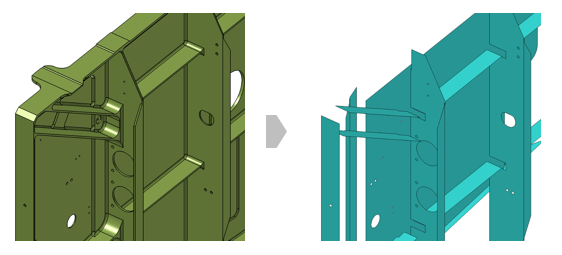
\includegraphics[width=0.7\linewidth]{..//Common/images/MidsurfaceErrorsMscApex}
%\caption{Midsurface by a  latest commercial application (Source:~\cite{MScApex})}
%\label{fig:midsurfaceerrors}
%\end{figure}

Following are some of the salient observations based on the literature survey done:
 
\begin{itemize}[noitemsep,topsep=2pt,parsep=2pt,partopsep=2pt]%leftmargin=*

	\item In feature based defeaturing approaches, full feature dimensions were used for selecting features for removal thereby giving wrong results.
	\item For defeaturing, application domain-specific rules of identification of features for removal are necessary instead of identification of any feature below the `threshold' size.
	\item Past midsurface generation approaches are limited in the range of input model geometries (say, only planar or analytic surfaces), feature types (say, only extruded, positive primitives) and connection types (say, only, parallel, or perpendicular) they could handle. Due to these limitations, the output midsurface has many errors, especially for complex input solid models.
	\item  %\textbf{Midsurface Patches Generation}:  \label{sec:facepairdetection}
In face pairing approaches, finding the face-pairs in a complex part itself is very challenging. Issues like, faces may not be directly opposite to each other, may not be parallel, may have multiple opposite faces, etc. are frequent. Such wrong face pairs result in gaps in the output midsurface. %This research addresses this problem by using the Abstracted feature-information for generation of patches and avoids detection of face-pairs  (more details in section~\ref{sec:scell}). 
	\item  %\textbf{Midsurface Patches Connection}: \label{sec:facepairinteraction}
For connecting midsurface patches, there is no definitive list of connection types. Thus providing deterministic logic is not possible. This limitation results in midsurface patches not being joined properly, resulting in gaps or overlaps. %This research proposes  leveraging of feature based cellular decomposition (more details in section~\ref{sec:icell}).
\end{itemize}
 
 %The proposed approach is `generic', meaning, in principle, no such restrictions are present in this approach. It can be made to cater to any geometry types, feature types or connections. Advantages can be seen in the range of shapes handled as well as in the minimization of failures (Section~\ref{sec:results}).
 


%Based on all the surveys done and observations, following research objectives were formulated for the present research work.

\deleted{{\bfseries Thus, so far, there has been a limited success in the objective of computing a well-connected midsurface. This research plans to leverage feature information to achieve this objective.}}

\section{Research Objectives} \label{sec:introduction:rs}

The overall objective of the proposed research is to develop a system to generate a quality midsurface of sheet metal feature based CAD model \added{by developing various algorithms}. \replaced{Based on the extensive literature survey and critical analysis, following research objective are laid down, as}{This objective is broken down further into following sub-objectives}:
\begin{itemize}[noitemsep,topsep=2pt,parsep=2pt,partopsep=2pt]
\item To develop \replaced{defeaturing algorithms to simplify CAD feature model as much as possible without impacting the gross shape of the part}{ and implement a feature based model simplification (defeaturing) approach to generate a ``gross shape'', which improves midsurface generation}.
\item To develop \replaced{algorithms to represent the feature based CAD model by transforming existing set of sheet metal features to a finite set of generalized features}{and implement a feature abstraction approach to further simplify the model, by transforming each feature to a generalized form, reducing the number of scenarios to handle}.
\item To develop \replaced{algorithms for generating quality midsurfaces leveraging generalized feature based CAD model and cellular decomposition covering a wide variety of topological connectivities}{and implement a generic midsurface generation approach leveraging generalized feature form and cellular decomposition}.
\item To \replaced{come up with an approach to topologically validate the generated midsurface relative to its input CAD  model}{develop a topological validation methodology to assess correctness of the midsurface}.
\item \replaced{To implement a software system incorporating above algorithms and }{To test real-life parts to} demonstrate the efficacy of the proposed approach.
\end{itemize}

\section{Research Methodology} \label{sec:introduction:rm}
The present research work uses empirical hypothesis testing research methodology. 

%%\bigskip

	\begin{figure} [!h]
		\centering
		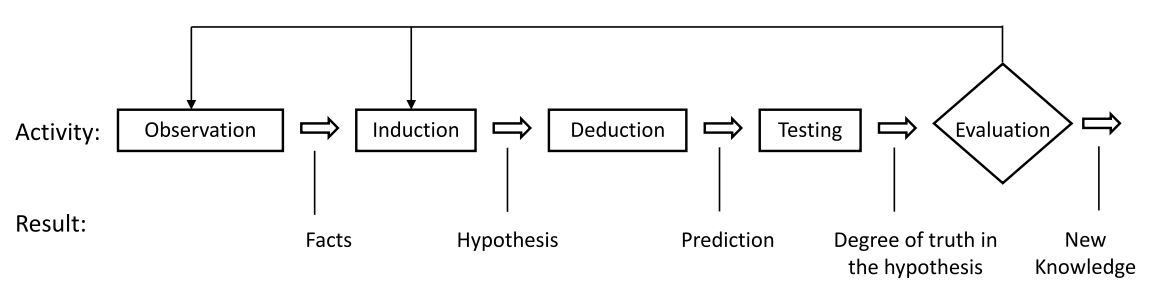
\includegraphics[width=0.9\linewidth]{..//Common/images/ResearchMethodology.png}
		\caption{Empirical Hypothesis Testing Process (Source: Stolt~\cite{Stolt2008})}
		\label{fig:introduction:ResearchMethodology}
	\end{figure}

%%\bigskip
	
Figure~\ref{fig:introduction:ResearchMethodology} shows the empirical hypothesis process and its various phases. Following paragraph explains them along with their interpretation in the context of present research work. 

The empirical hypothesis testing process starts with observations, e.g. the problems observed in the current midsurface generation approaches. These facts are generalized by induction into a hypothesis, such as, the core problems in midsurface extraction are detection of sub-shapes and interactions amongst them. Predictions are then deduced from the hypothesis, such as, if the input model is simplified, generalized and decomposed, the problem could be more deterministic to handle.  A prototype is built incorporating the proposed solution. After testing the prototype, if the results are valid and acceptable, then the hypothesis is accepted as true for the time being. In the present research work, hypothesis takes the form of a set of multiple sub-hypotheses and the proposed system answers those questions. Section~\ref{sec:litsurvey:rquestions} lists the hypothesis whereas Chapter~\ref{ch:Proposal} presents the proposed system.

 \section{Research Scope}
The proposed research aims at developing algorithms for generating a quality midsurface of thin-walled \added{sheet metal} feature based CAD model. \deleted{Domain selected is of sheet metal parts.} Reason for \replaced{considering sheet metal parts in scope}{selection} is due to its wide usage in domains ranging from household items to big ships.  Better midsurface will have an enormous impact on quicker and robust product development in all these domains.

\todo{Review comment: May need concrete justification. [DONE]}

%Sheet metal models are unique in both, geometrical and topological sense. They are characterized by:
%\begin{itemize}[noitemsep,topsep=2pt,parsep=2pt,partopsep=2pt]
%\item \textbf{Constant thickness}: Made up of constant thickness blank roll.
%\item \textbf{Absences}: There are no blind holes, but only through holes, if any. 
%\item \textbf{Degeneracy}: There are no degenerate capping thickness faces (like ``Wedge'').
%\item \textbf{Cavities}: There are no embedded volumes or cavities (``bubbles'').
%\end{itemize}
%%%CAD models of sheet metal parts use a wide variety of feature such as~\cite{Liu2004} (Figure~\ref{liuFeatures}):
%%%
%%%	\begin{figure} [!h]
%%%		\centering
%%%		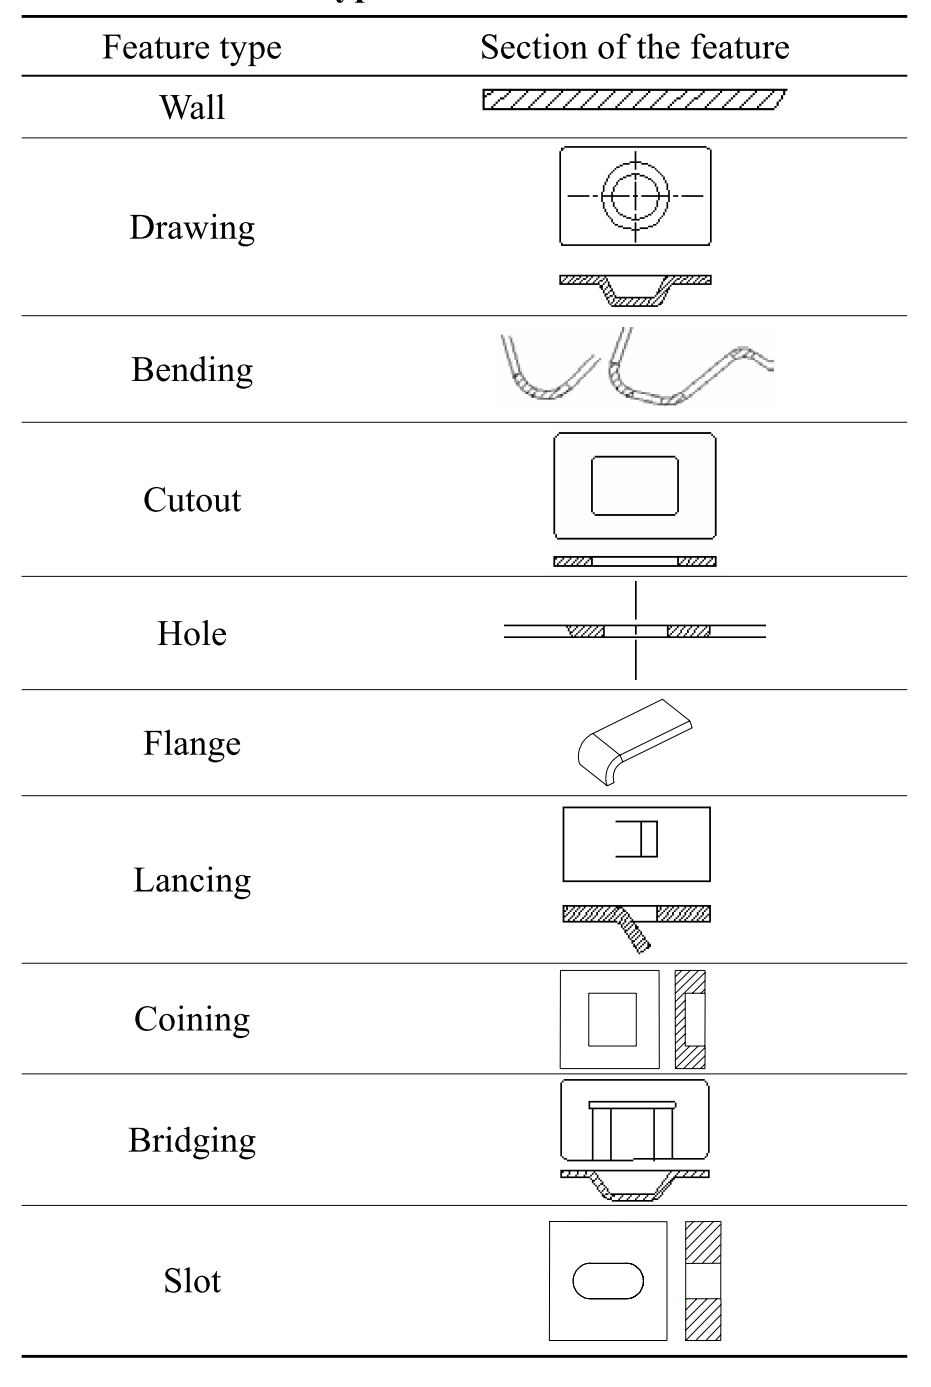
\includegraphics[width=0.6\linewidth]{..//Common/images/liuFeatures}
%%%		\caption{Typical Sheet metal features~\cite{Liu2004}}
%%%		\label{fig:liufeatures}
%%%	\end{figure}
%	
%	
%\begin{minipage}[c]{0.98\linewidth}
%\begin{minipage}[t]{0.48\linewidth}
%\begin{itemize}[noitemsep,topsep=2pt,parsep=2pt,partopsep=2pt]
%\item \textbf{Primitive features}: These features an exist interdependently and form primary shape of the part, e.g. Wall, Drawing.
%\item \textbf{Add-on features}: These features must be added to the existing features and are secondary in nature, e.g. Cutout, Hole, Slot.
%\item \textbf{Connecting features}: These features act as a bridge between other features, e.g. Bend.
%\item \textbf{Composite features}: These are feature collections, .e.g. Array.
%\end{itemize}
%\end{minipage}
%\hfill
%\begin{minipage}[t]{0.48\linewidth}
%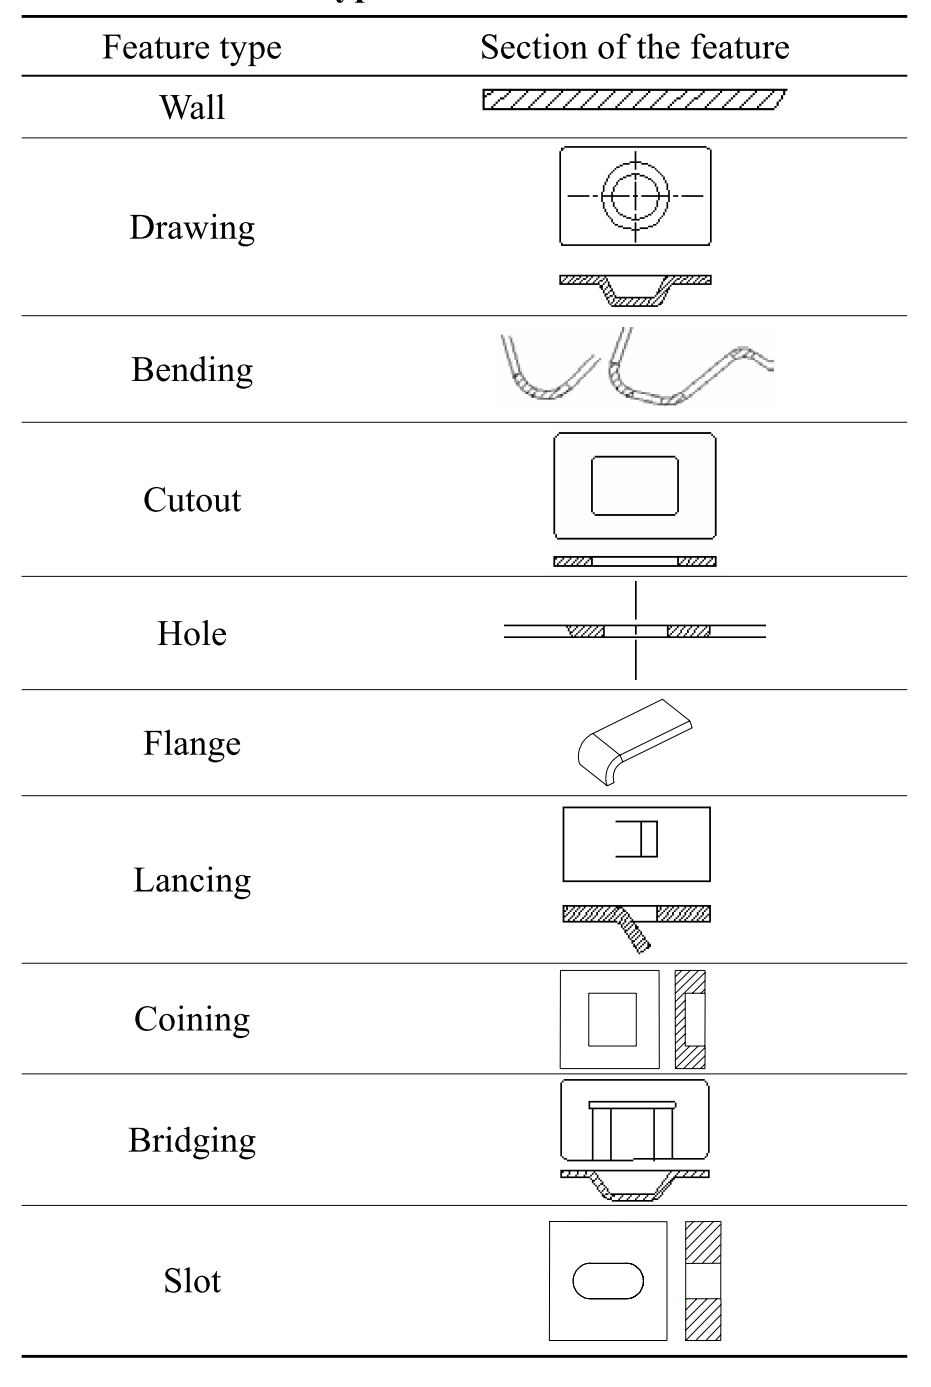
\includegraphics[width=0.52\linewidth,valign=t]{..//Common/images/liuFeatures}
%\captionof{figure}{Typical Sheet metal features~\cite{Liu2004}}\label{fig:liufeatures}
%\end{minipage}
%\end{minipage}
\added{The proposed system accepts feature based CAD model built using Autodesk Inventor\textsuperscript{\textregistered}, as input. Thus, the feature based alogirthms devised in the present research, work on sheet metal features, such as, Walls, Flanges, Bends, Cutouts, etc.}
\deleted{The proposed system works on the sheet metal feature based CAD models as input, having features similar to ones mentioned above. In particular, it caters to parts made by fabrication, which show significant problems in generating midsurface, especially at the joints. It should be possible to extend it to variable-thickness components as well, with further customizations.}
\added{Autodesk Inventor\textsuperscript{\textregistered} was chosen over other CAD systems, such as Solidworks, Parametric Creo, etc. due to its free availability for students and maturity of APIs.}

Following section lists hypotheses tested by the present research work.

\section{Research Hypotheses} \label{sec:litsurvey:rquestions}

%Based on the study so far, the present research proposes a new paradigm, called ``F-SAD'' ({\bf F}eature-based, {\bf S}implification, {\bf A}bstraction, {\bf D}ecomposition), leverages use of features, simplification, abstraction and decomposition as a general approach to be used in the development of CAD functionalities. 
This research proposes following hypotheses and assesses them against the proposed system.% So, hypotheses that are going to be tested  are:

\begin{myhyp}
\label{hyp:features}
Instead of working on a Brep CAD model as input, the feature based CAD model enables computation of a well-connected midsurface.
\end{myhyp}

\begin{myhyp}
\label{hyp:Simplification}
Instead of working on a detailed CAD model, the defeatured model results in a better midsurface.
\end{myhyp}

\begin{myhyp}
\label{hyp:Abstraction}
Instead of working on a wide variety of features, the generalized feature representation helps devise a generic midsurface patch computation algorithm, thus avoiding problems of face pairing.
\end{myhyp}

\begin{myhyp}
\label{hyp:Decomposition}
Instead of working on a full CAD model, the decomposed model helps devise a generic midsurface patch joining algorithms, thus avoiding problems of gaps and overlaps in the midsurface.
\end{myhyp}

\begin{myhyp}
\label{hyp:MidsurfaceComputation}
Feature based defeaturing, generalization and decomposition, together help compute a well-connected midsurface.
\end{myhyp}

\todo{Review comment: Add 2-3 lines after this. [DONE]}

\added{This chapter has presented review of the past approaches for generating midsurface along with the associated techniques of defeaturing. It summarized the observations and presented the objectives for the present research. The following chapter will present the proposed system to address the research objectives.}

%\added{This chapter has presented the overview of MIDAS, the proposed system to compute a well-connected midsurface from feature-based sheet metal CAD part model. Following chapters present various modules in details. Last chapter demonstrates the capabilities of MIDAS with reference to the typical component case studies.}

%
%\subsection{Sheet Metal Features Taxonomy} \label{sec:litsurvey:rscope}
%
%\subsection{Rsearch Questions to be answered in this thesis} \label{subsub:questions}
%This work attempts to answer following questions:
%\begin{itemize}[noitemsep,topsep=2pt,parsep=2pt,partopsep=2pt,leftmargin=*]
%\item How to simplify a thin-walled part so as to improve chances of getting a wellc-connected midsurface?
%\item How to abstract features so as to reduces cases for computation of midsurface patches?
%\item How to compute a well-connected midsurface using a generic logic?
%\item How to validate quality of a midsurface?
%\end{itemize}

